% Created with jtex v.1.0.17
\documentclass{article}
\PassOptionsToPackage{short, nodayofweek}{datetime}


% Start Curvenote Definitions

% Pass Options Section
% base
\PassOptionsToPackage{normalem}{ulem}
\PassOptionsToPackage{utf8}{inputenc}

% template
\PassOptionsToPackage{framemethod=TikZ}{mdframed}
\PassOptionsToPackage{x11names, svgnames}{xcolor}

%%% PACKAGES

% base
\usepackage{inputenc}
\usepackage{url}
\usepackage{graphicx}
\usepackage{adjustbox}
\usepackage{amssymb}
\usepackage{amsfonts}
\usepackage{amsmath}
\usepackage{enumitem}
\usepackage{nicefrac}
\usepackage{booktabs}
\usepackage{microtype}
\usepackage{hyperref}
\usepackage{ulem}
\usepackage{enumitem}
\usepackage{float}
\usepackage{datetime}
\usepackage{xkeyval}
\usepackage{framed}
\usepackage{doi}

% template
\usepackage{natbib}
\usepackage{fancyvrb}
\usepackage{mdframed}
\usepackage{xcolor}

%%%


%%%% Setup Section

% base
\graphicspath{{.}}
% template
\sloppy
\newenvironment{aside}{\begin{framed}}{\end{framed}}
\newmdenv[linewidth=2pt,linecolor=CornflowerBlue,topline=false,bottomline=false,rightline=false,leftline=true,skipabove=20,skipbelow=20,leftmargin=20,rightmargin=20]{callout}
\newfloat{code}{thp}{loc}
\floatname{code}{Program}
\raggedbottom
\bibliographystyle{abbrvnat}
\setcitestyle{authoryear,open={(},close={)},semicolon,aysep={,}}

% End Curvenote Definitions




% colors for hyperlinks
\hypersetup{colorlinks=true, allcolors=blue}
\hypersetup{
pdftitle={\@title},
pdfsubject={},
pdfauthor={\@author},
pdfkeywords={},
addtopdfcreator={Written in Curvenote}
}

\usepackage{curvenote}

\title{Twin experiments to test DA}

\newdate{articleDate}{12}{6}{2024}
\date{\displaydate{articleDate}}

\author{}

\begin{document}

\maketitle
\keywords{}

This project aims to validate and assess the effectiveness of data assimilation (DA) techniques by conducting a twin experiment with:

\begin{itemize}
\item Soil moisture content (SMC) data
\item Electrical Resistivity Tomography (ERT) 2d profiles
\item Actual Evapotranspiration(ET) from EO (Earth Observations)
\end{itemize}

\textbf{True State Generation}
The true state of soil moisture is generated by running a hydrological model with \textbf{known parameters and forcing data} over a 24-hour period. This true state serves as the synthetic reality for the experiment.

\begin{figure}[!htbp]
\centering
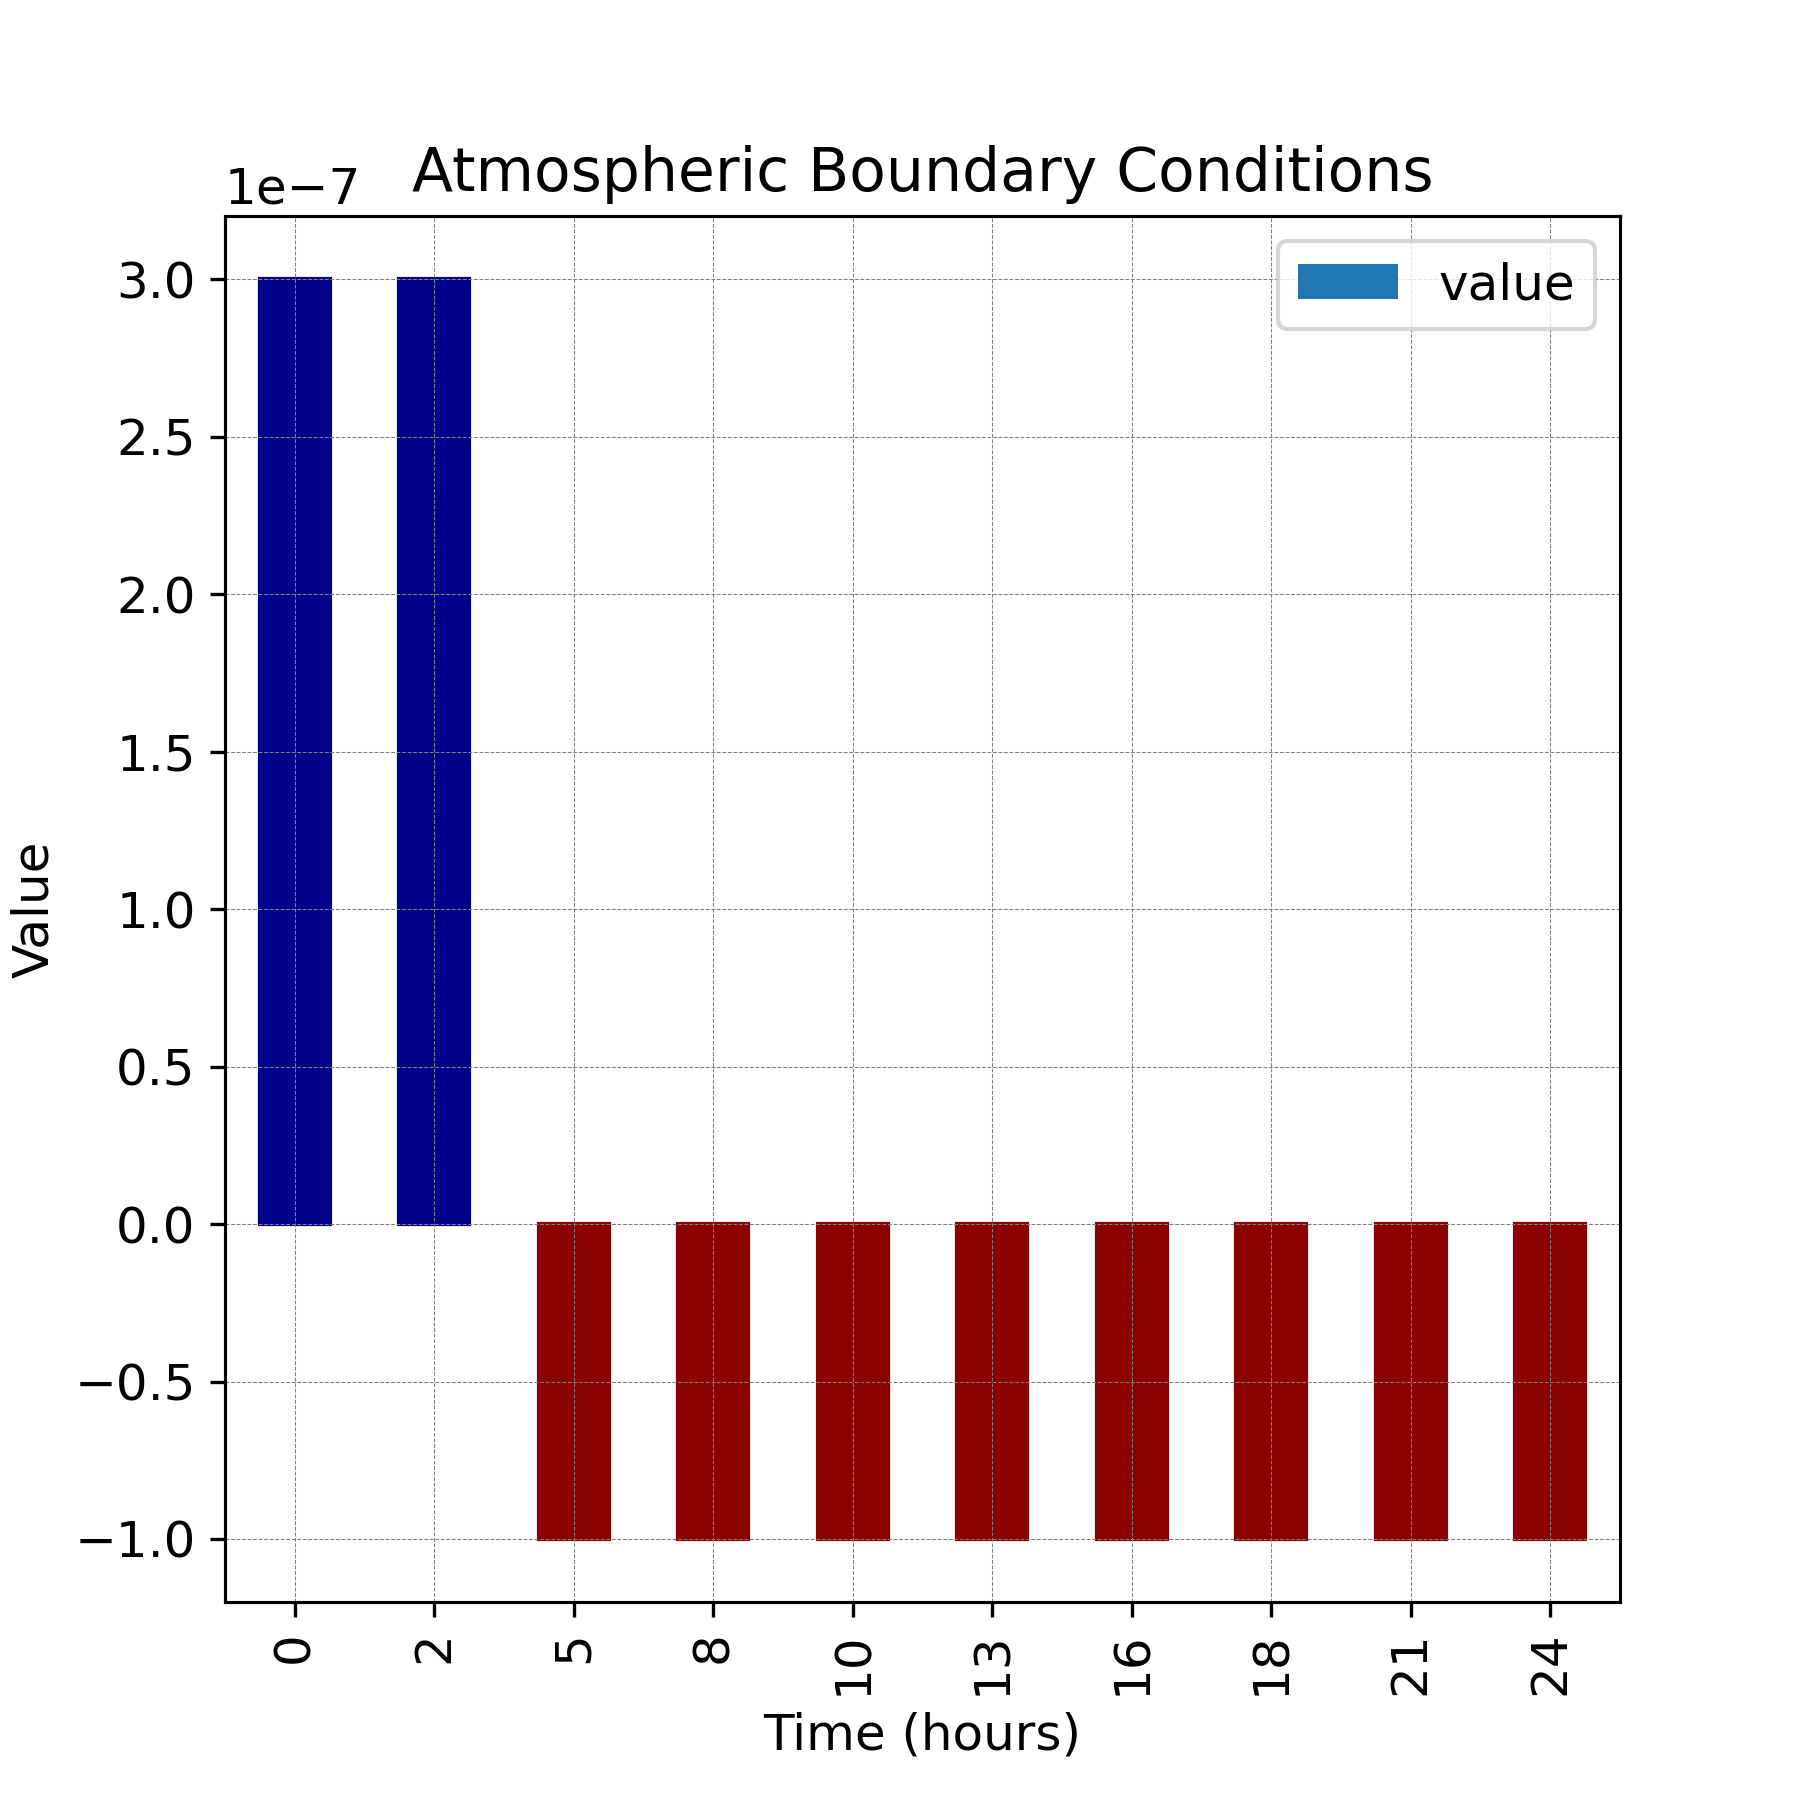
\includegraphics[width=0.75\linewidth]{files/atmbc-f09b5504b84b8c8eec07ec45739288f2.png}
\caption[]{True-state-atmbc}
\label{true-state-atmbc}
\end{figure}

\begin{figure}[!htbp]
\centering
\includegraphics[width=0.75\linewidth]{files/vtksaturation_slow-3db06418d1bd02216f096b66d7fed8a1.gif}
\caption[]{True state generation for soil moisture over a 24-hour period.}
\label{true-state-figure}
\end{figure}

\textbf{Perturbed Initial State}
A new simulation of the hydrological model is initiated with perturbed initial conditions and/or parameters. This represents the model's initial guess, which deviates from the true state.

\begin{figure}[!htbp]
\centering
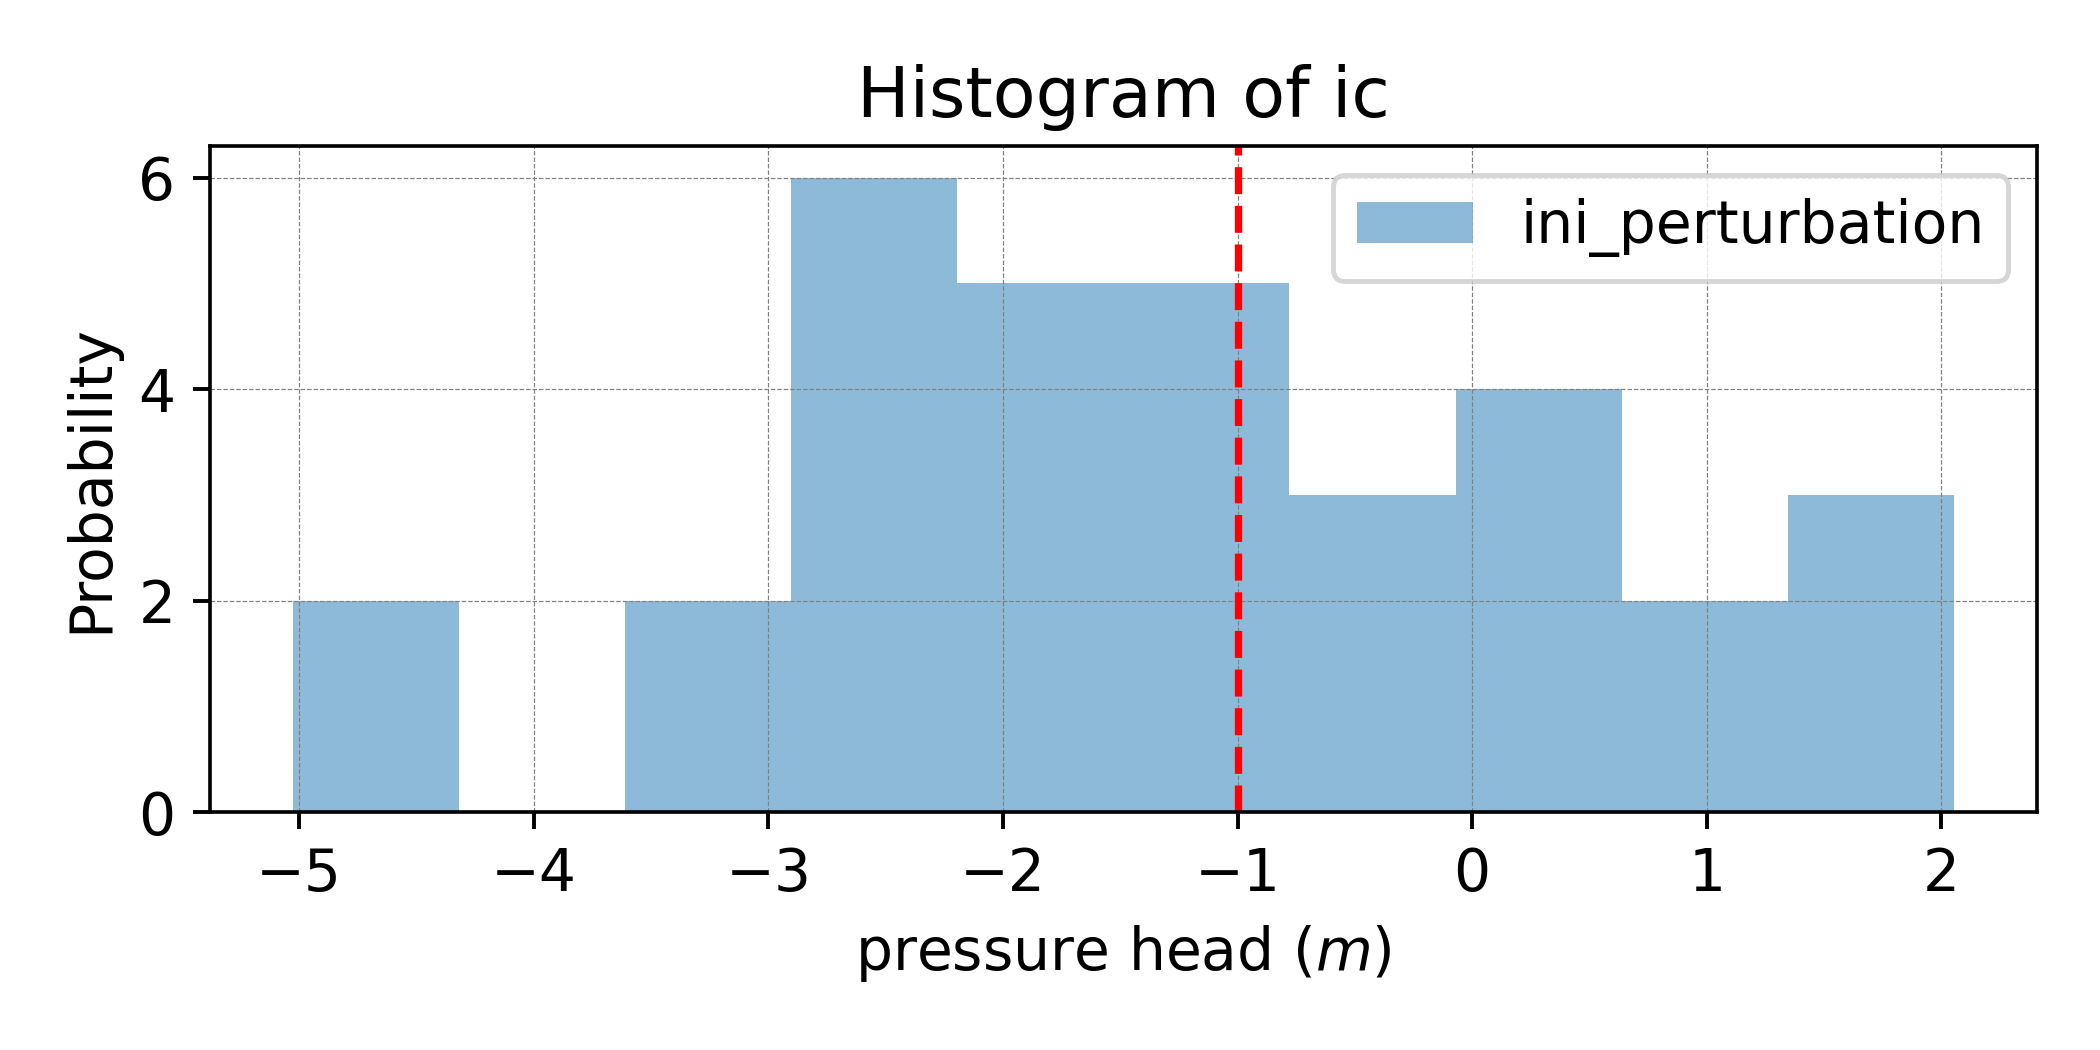
\includegraphics[width=0.75\linewidth]{files/meshLi_withDA_icic-945c2a46b18c7e738c0e57931a8949e2.png}
\caption[]{meshLi\_withDA\_ZROOT\_WITH\_UPDATEZROOT0}
\label{meshLi_withDA_ZROOT_WITH_UPDATEZROOT0}
\end{figure}

\begin{figure}[!htbp]
\centering
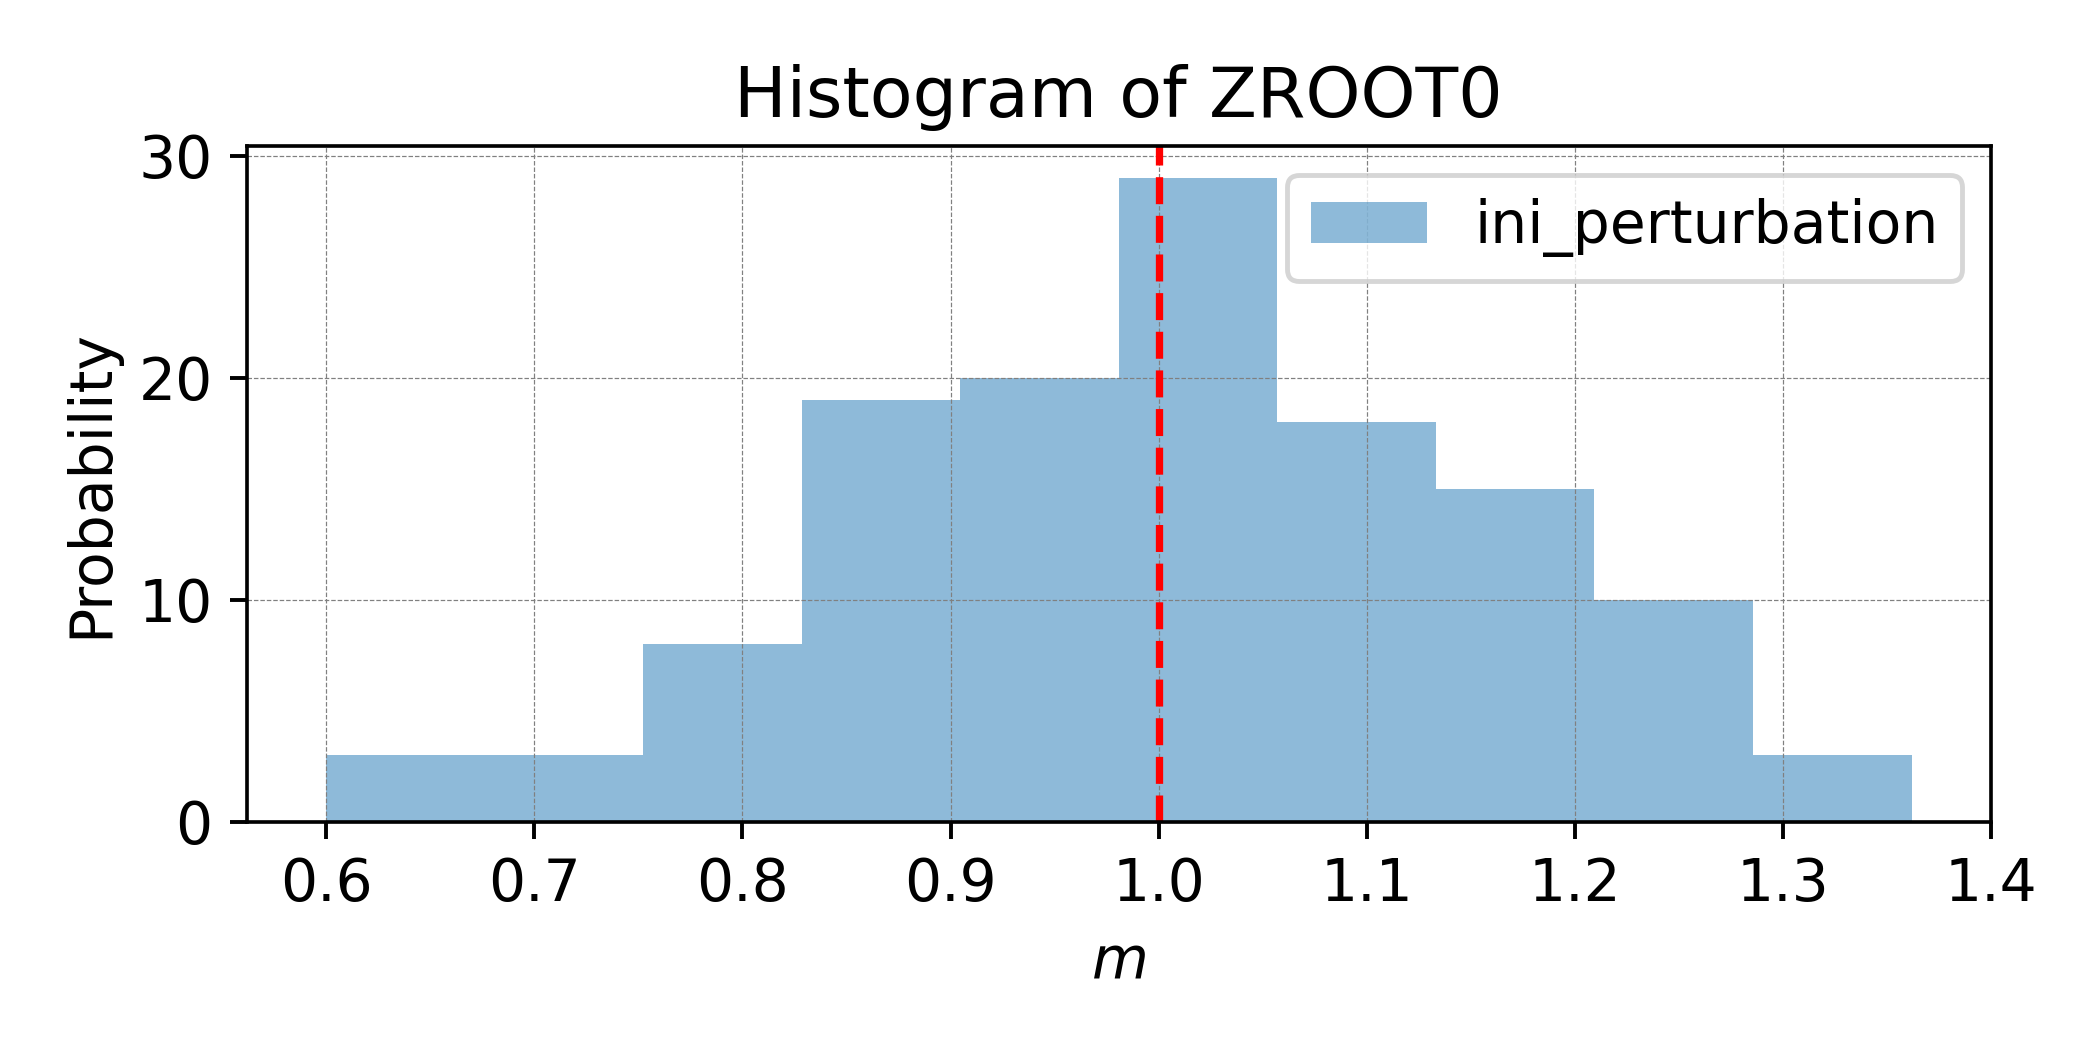
\includegraphics[width=0.75\linewidth]{files/meshLi_withDA_ZROOT_-2d60d7a9cb7a157f54335311b88f7e2e.png}
\caption[]{meshLi\_withDA\_ZROOT\_WITH\_UPDATEZROOT0}
\label{meshLi_withDA_ZROOT_WITH_UPDATEZROOT0}
\end{figure}

\textbf{Data Assimilation}
The synthetic observations are assimilated into the hydrological model using the Ensemble Kalman Filter (EnKF) method. This process updates the model state to better match the observations.

\textbf{Analysis and Evaluation}
The performance of the data assimilation is evaluated by comparing the assimilated model state with the true state. Metrics such as root mean square error (RMSE) are used to quantify the accuracy of the assimilation.

\section{SMC at 3 depths}

In this experiment, synthetic observations of soil moisture at three different depths are assimilated into a hydrological model every hour over a 24-hour period. Noise is added to the true solution to simulate real-world observation inaccuracies. A 5\% Gaussian noise is added to these observations to mimic measurement errors.

\subsection{Initial conditions perturbations}

\begin{figure}[!htbp]
\centering
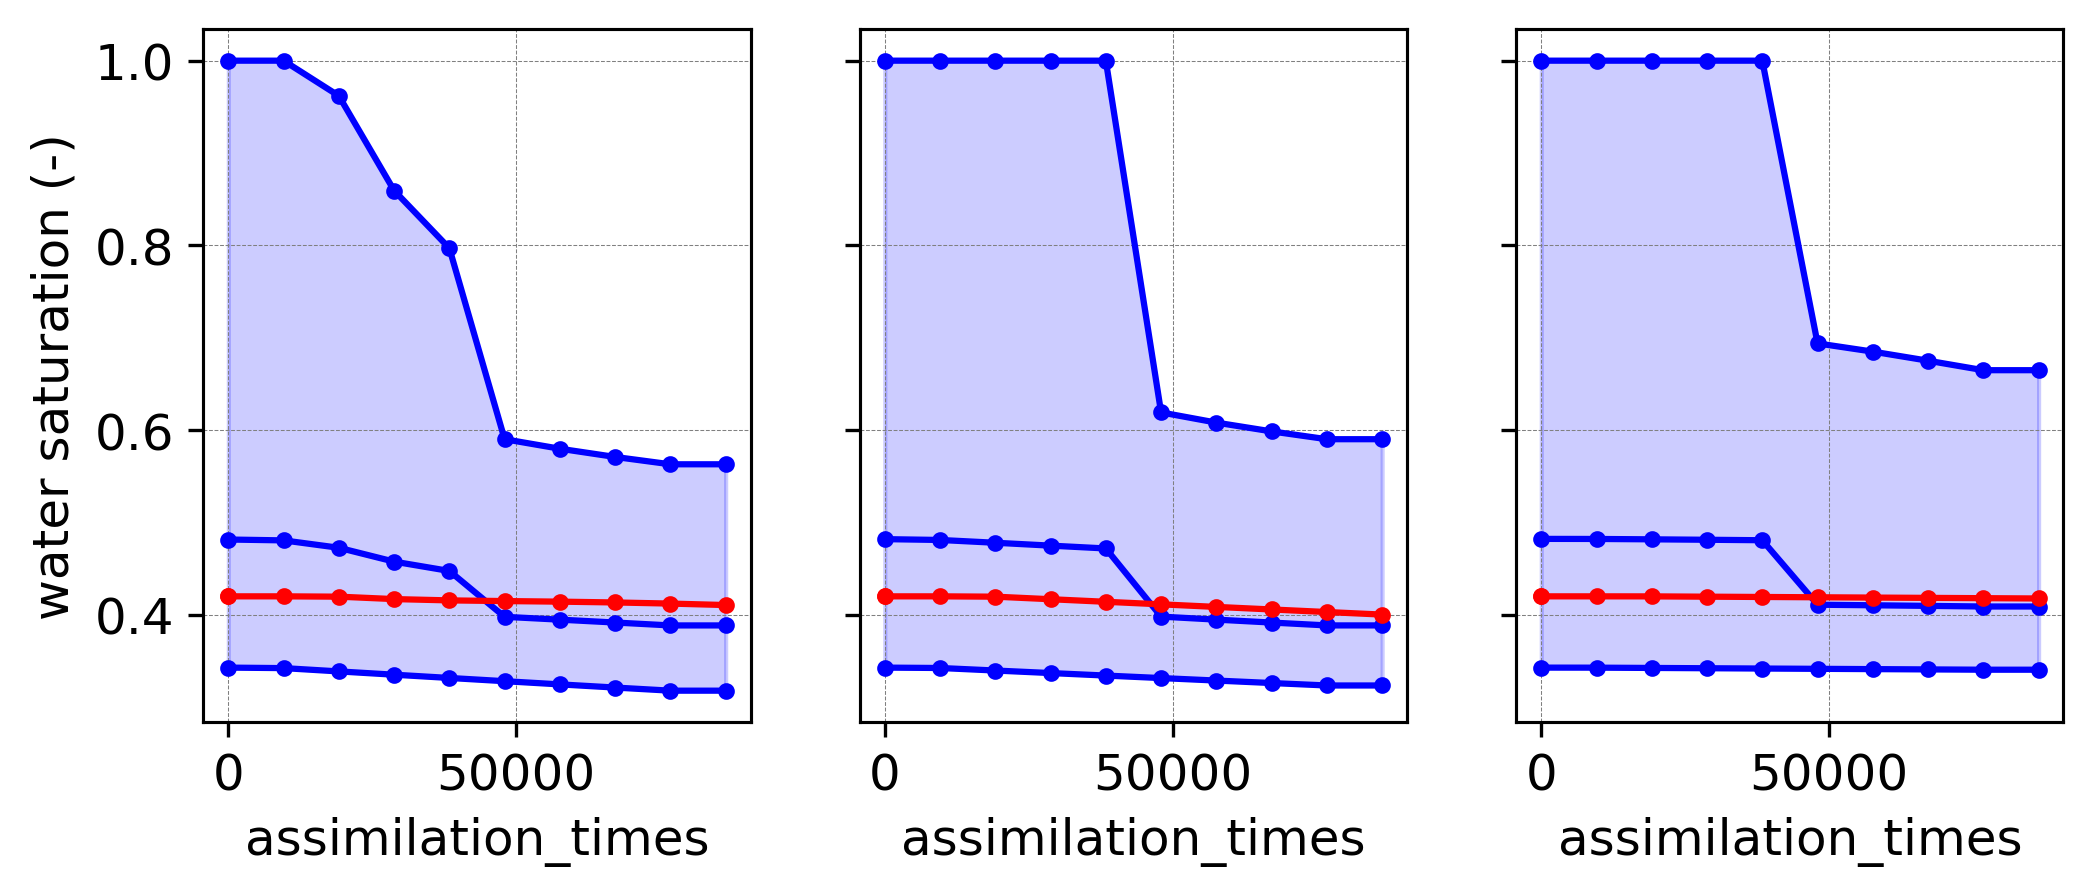
\includegraphics[width=0.75\linewidth]{files/SMC_withoutDA_ic_sw-80a4d7cd7a646d6d44550de4ab607d6f.png}
\caption[]{SMC\_withoutDA\_icsw}
\label{SMC_withoutDA_icsw}
\end{figure}

\begin{figure}[!htbp]
\centering
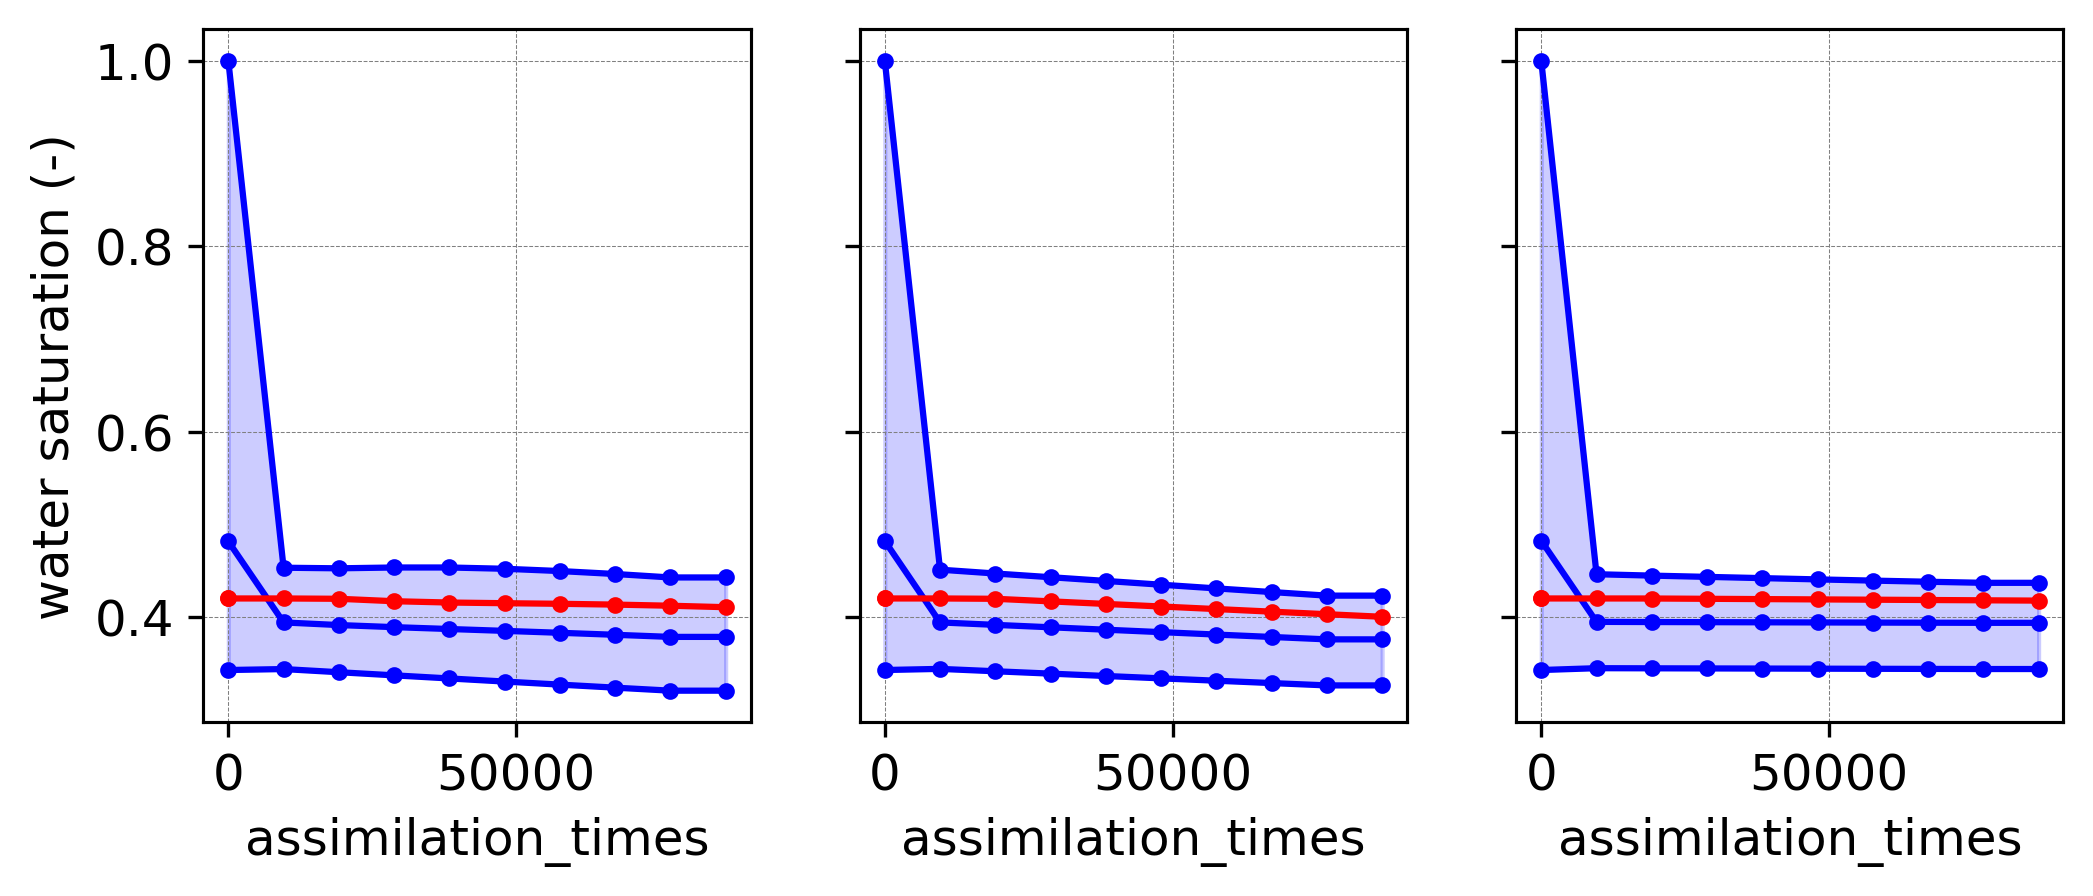
\includegraphics[width=0.75\linewidth]{files/SMC_withDA_ic_sw-4b08039f0ddf005f34bc3929ec4fefeb.png}
\caption[]{SMC\_withDA\_icsw}
\label{SMC_withoutDA_icsw}
\end{figure}

\subsection{Root depth perturbations and update}

\begin{figure}[!htbp]
\centering
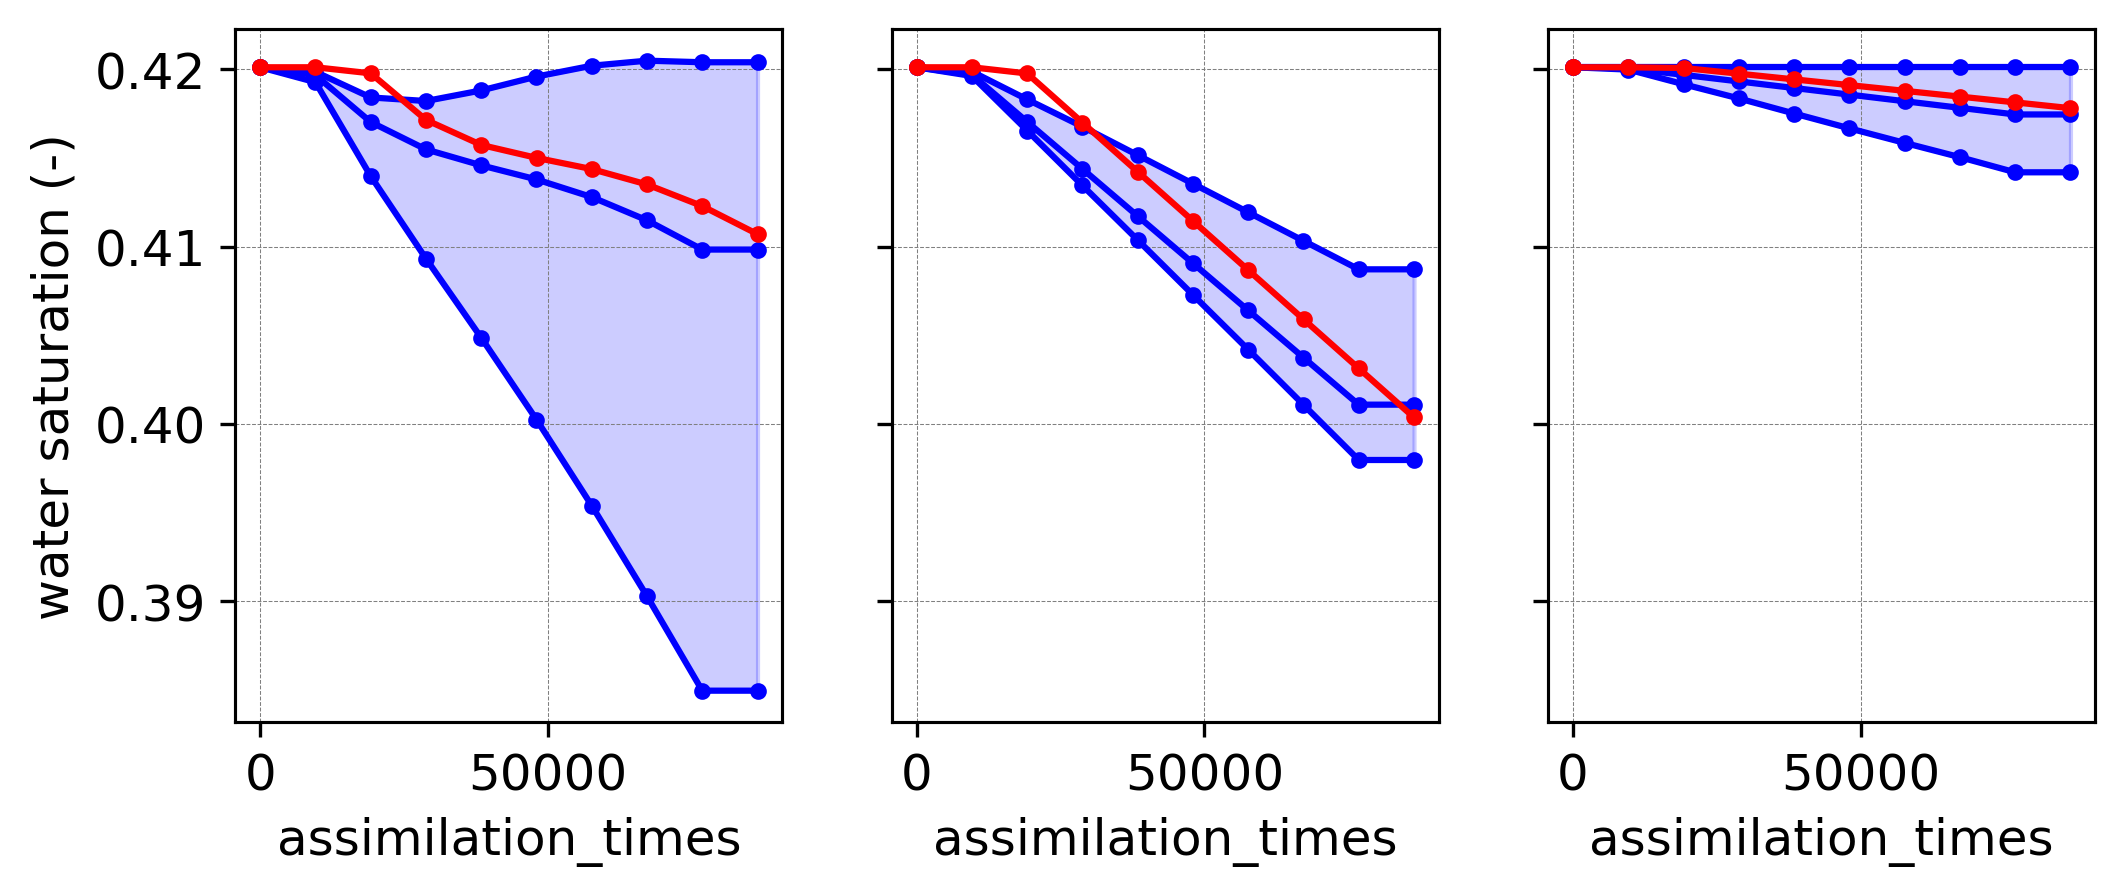
\includegraphics[width=0.75\linewidth]{files/SMC_withoutDA_ZROOT_-fdc0edfd18f4c02d3995e9d326740a27.png}
\caption[]{SMC\_withoutDA\_icsw}
\label{SMC_withoutDA_icsw}
\end{figure}

\begin{figure}[!htbp]
\centering
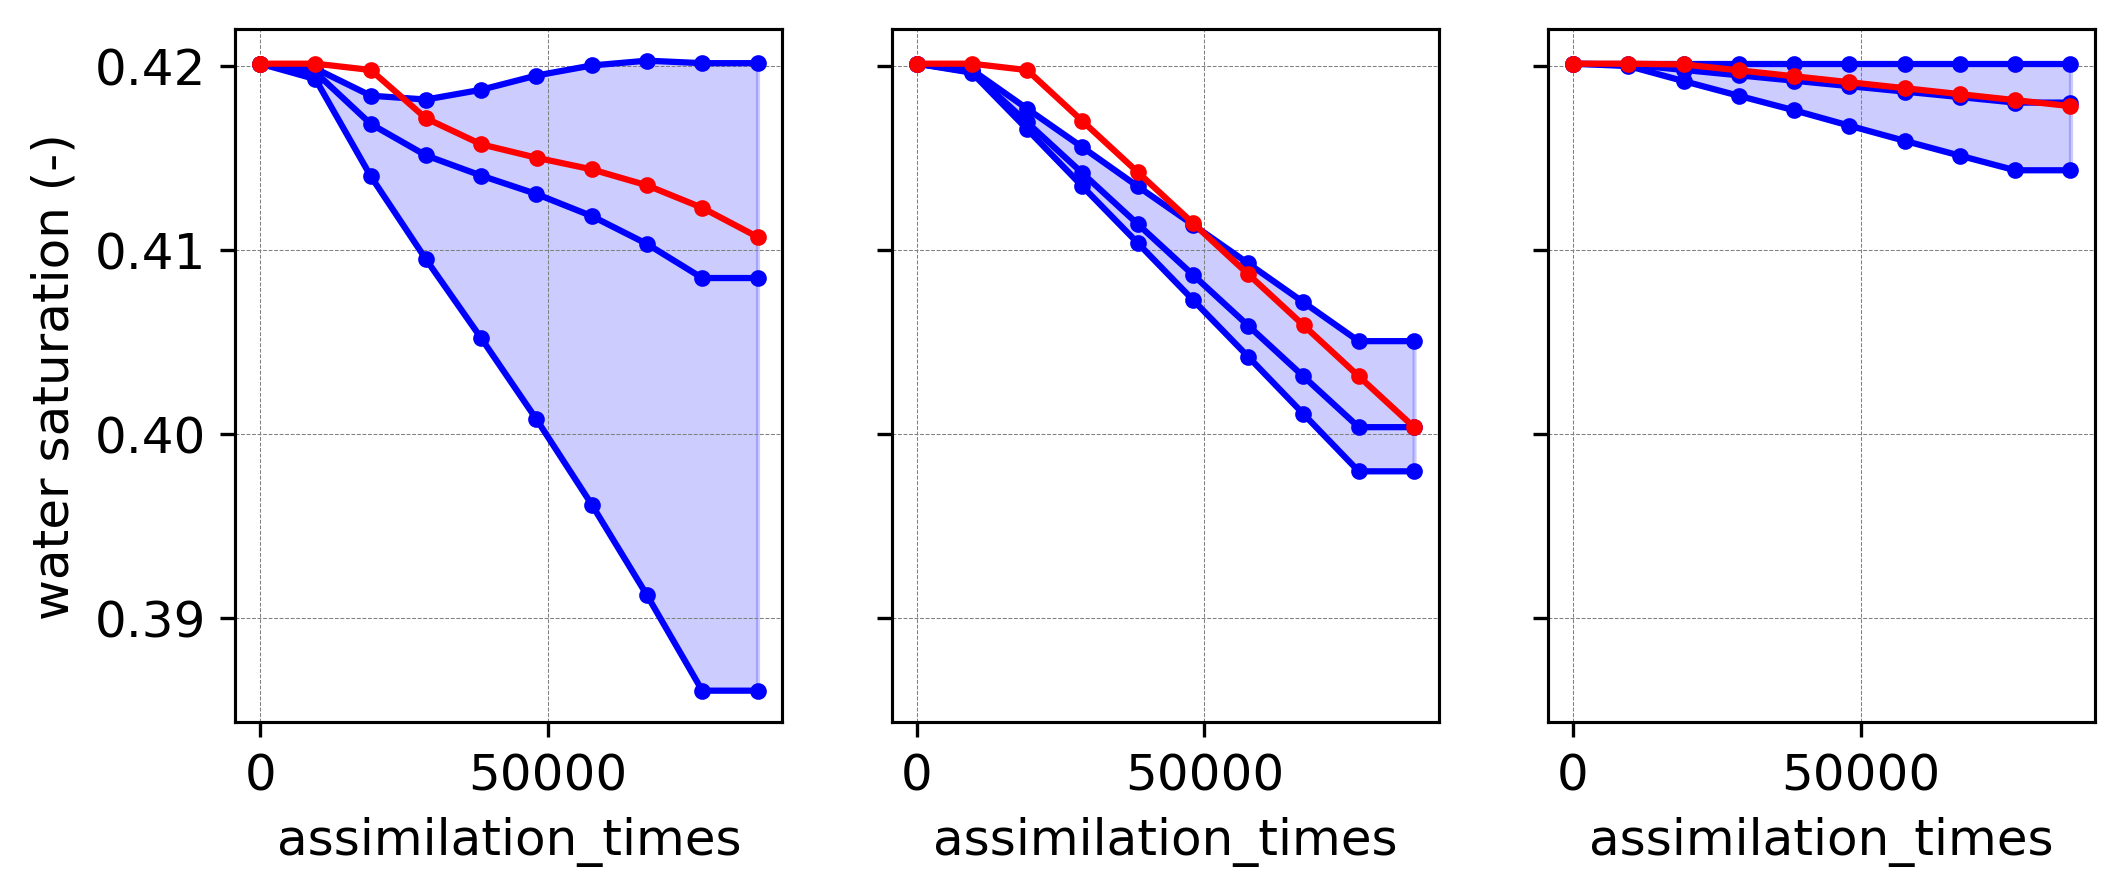
\includegraphics[width=0.75\linewidth]{files/SMC_withDA_ZROOT_WIT-b4d213075b05e8e7bc5bdf9a8bd60f8a.png}
\caption[]{SMC\_withDA\_icsw}
\label{SMC_withoutDA_icsw}
\end{figure}

\section{ERT 2d profiles}

\begin{figure}[!htbp]
\centering
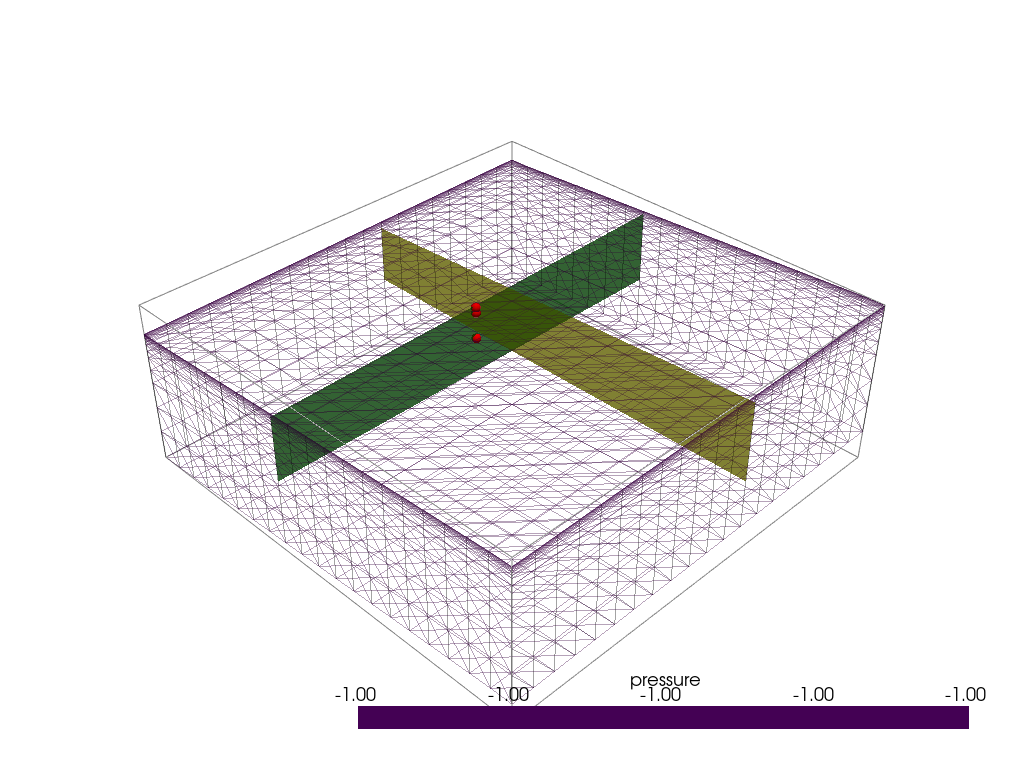
\includegraphics[width=0.75\linewidth]{files/meshERT-b7cdcd3033622116ec8ebebe7403f064.png}
\caption[]{meshERT}
\label{meshERT}
\end{figure}

\subsection{Initial conditions perturbations}

\begin{verbatim}
[scenario.ic]
per_type = ["None"]
per_name = ["ic"]
per_nom = [ -1]
per_mean = [ -1]
per_sigma = [1.75]
per_bounds = ["None"]
sampling_type = ["normal"]
transf_type = ["None"]
listUpdateParm = ["St. var."]
\end{verbatim}

\begin{figure}[!htbp]
\centering
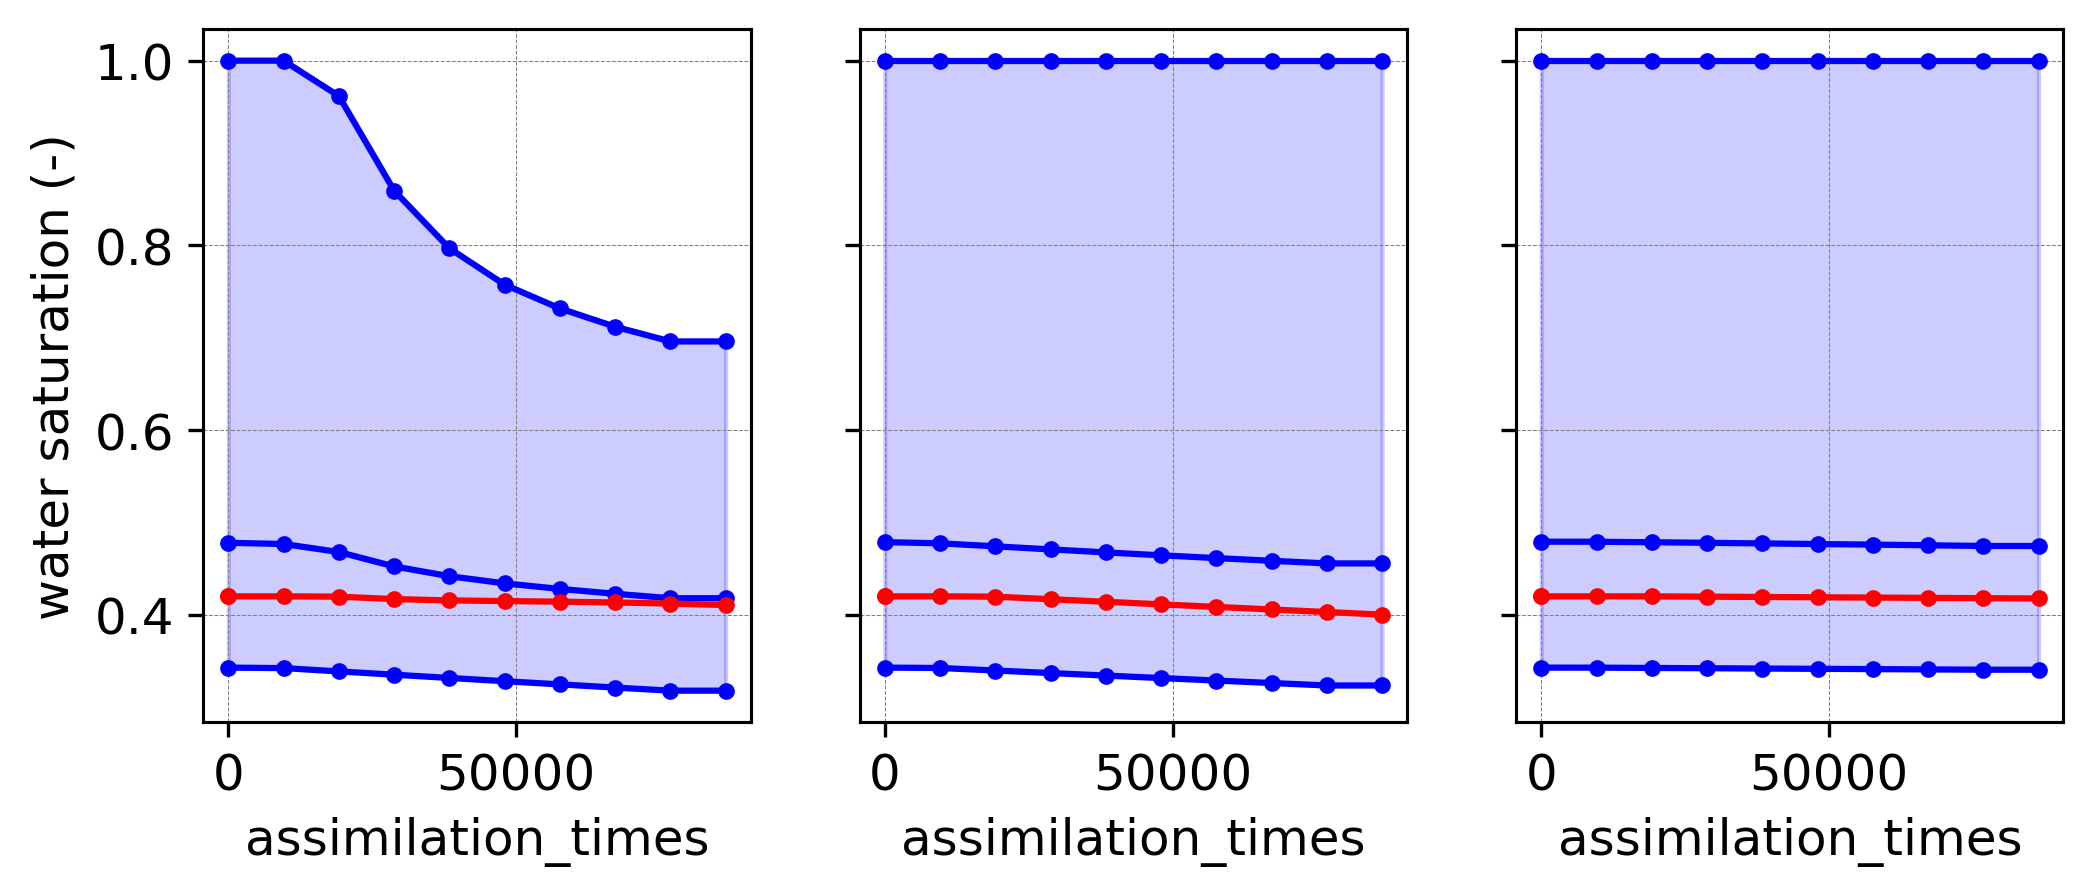
\includegraphics[width=0.75\linewidth]{files/meshLi_withoutDA_ic_-3288cd0f84d52e9dc3649e5deb9ae837.png}
\caption[]{meshLi\_withoutDA\_ic\_sw}
\label{meshLi_withoutDA_ic_sw}
\end{figure}

\begin{figure}[!htbp]
\centering
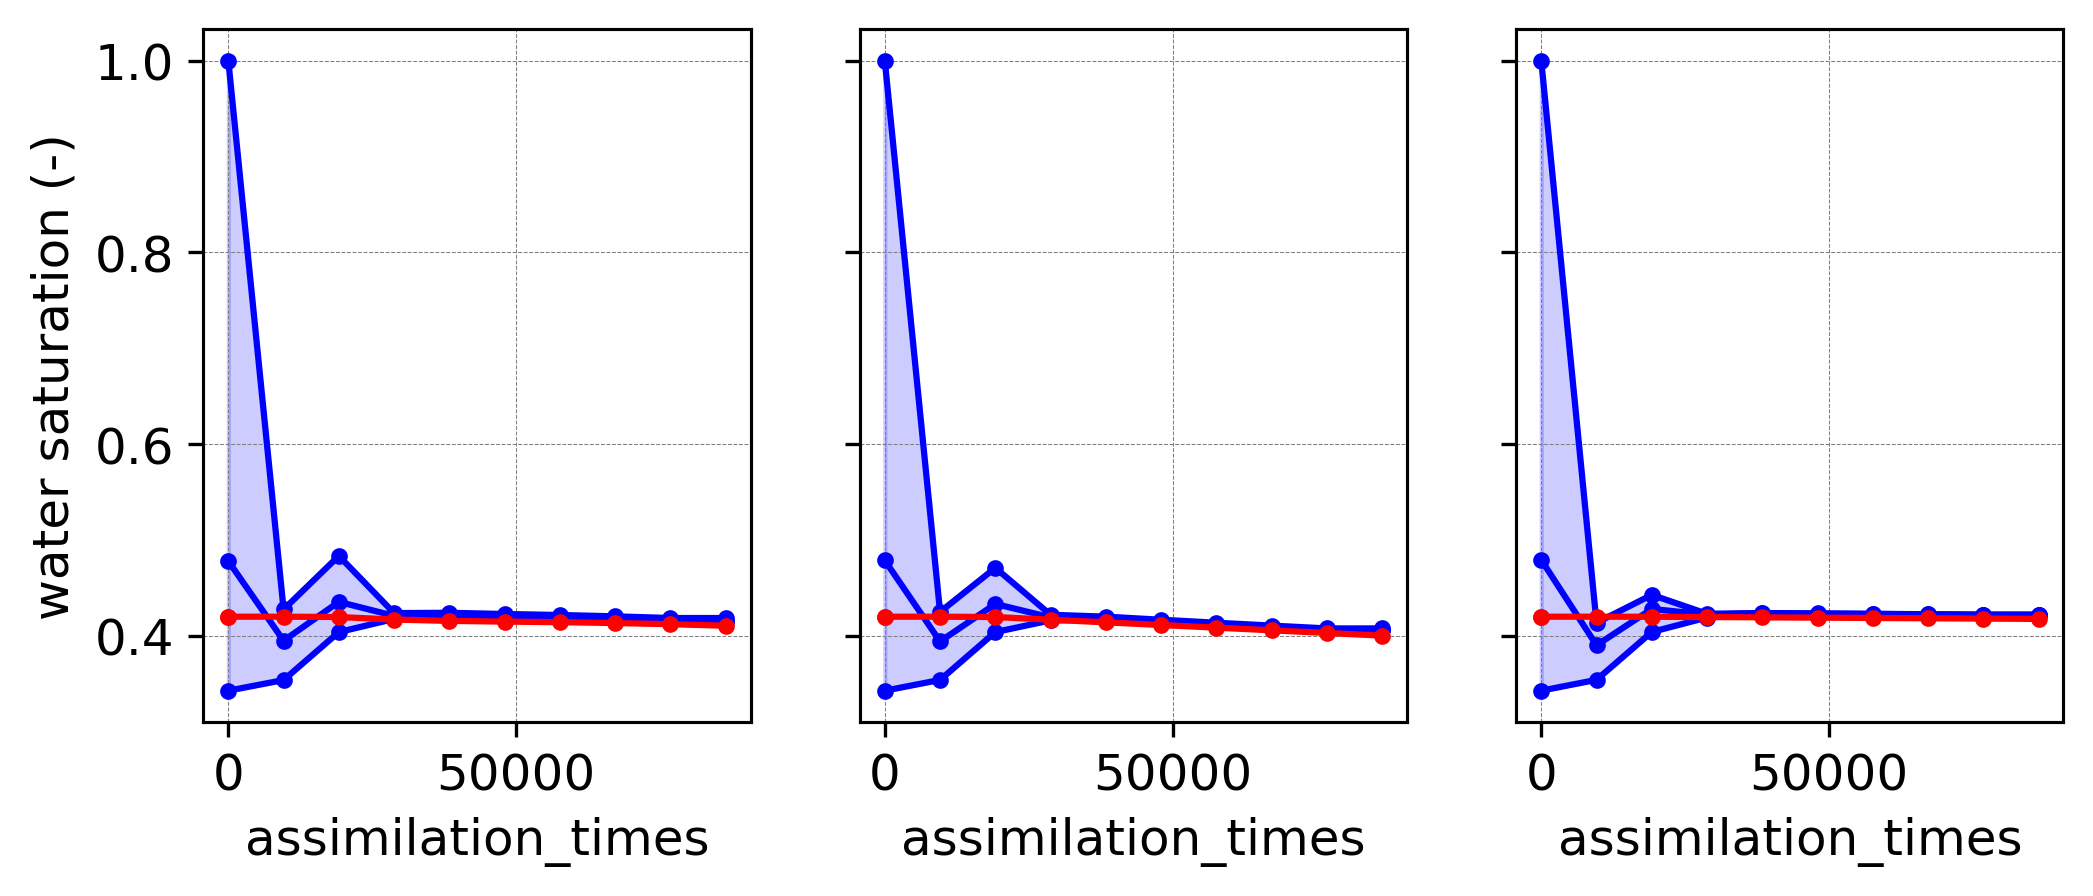
\includegraphics[width=0.75\linewidth]{files/meshLi_withDA_ic_sw-c3ce6044a7767982dea7f9f70b94f4fb.png}
\caption[]{meshLi\_withDA\_ic\_sw}
\label{meshLi_withDA_ic_sw}
\end{figure}

\subsection{Root depth perturbations and update}

\begin{figure}[!htbp]
\centering
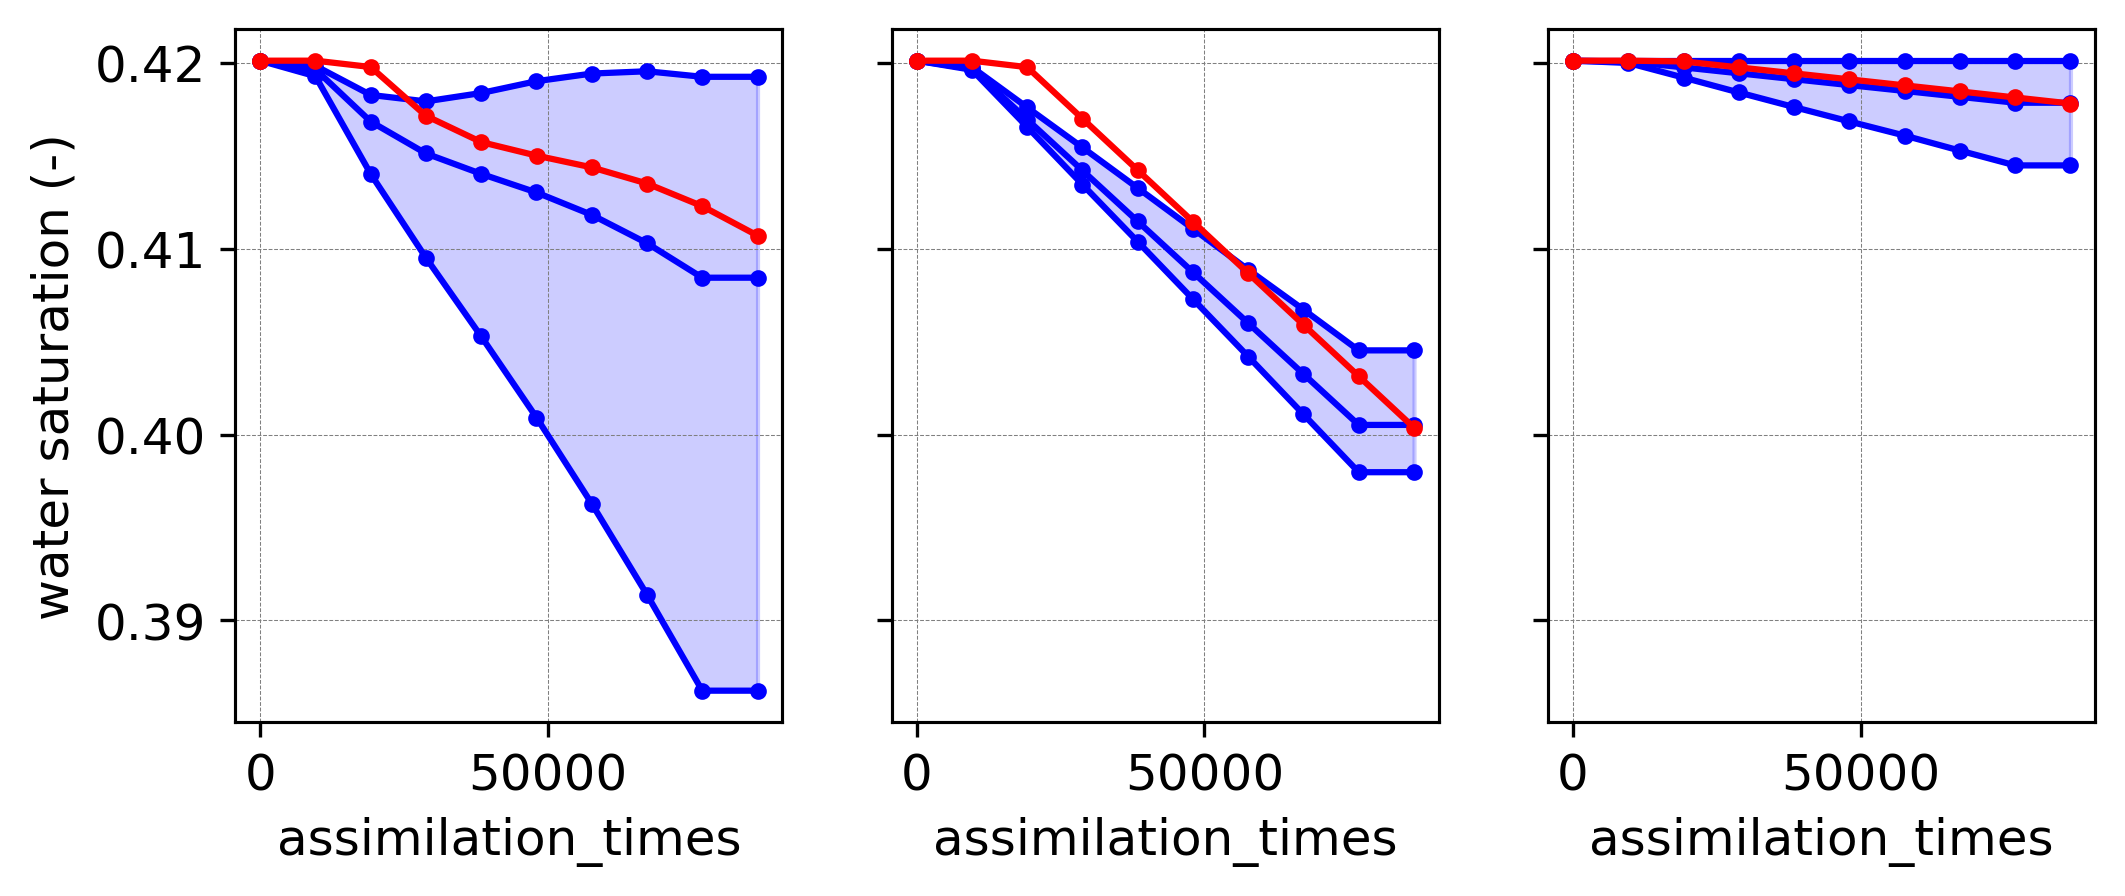
\includegraphics[width=0.75\linewidth]{files/meshLi_withoutDA_ZRO-a10db030e89a1da4fbac99c3d1316f71.png}
\caption[]{meshLi\_withoutDA\_ZROOT\_WITH\_UPDATE\_sw}
\label{meshLi_withoutDA_ZROOT_WITH_UPDATE_sw}
\end{figure}

\begin{figure}[!htbp]
\centering
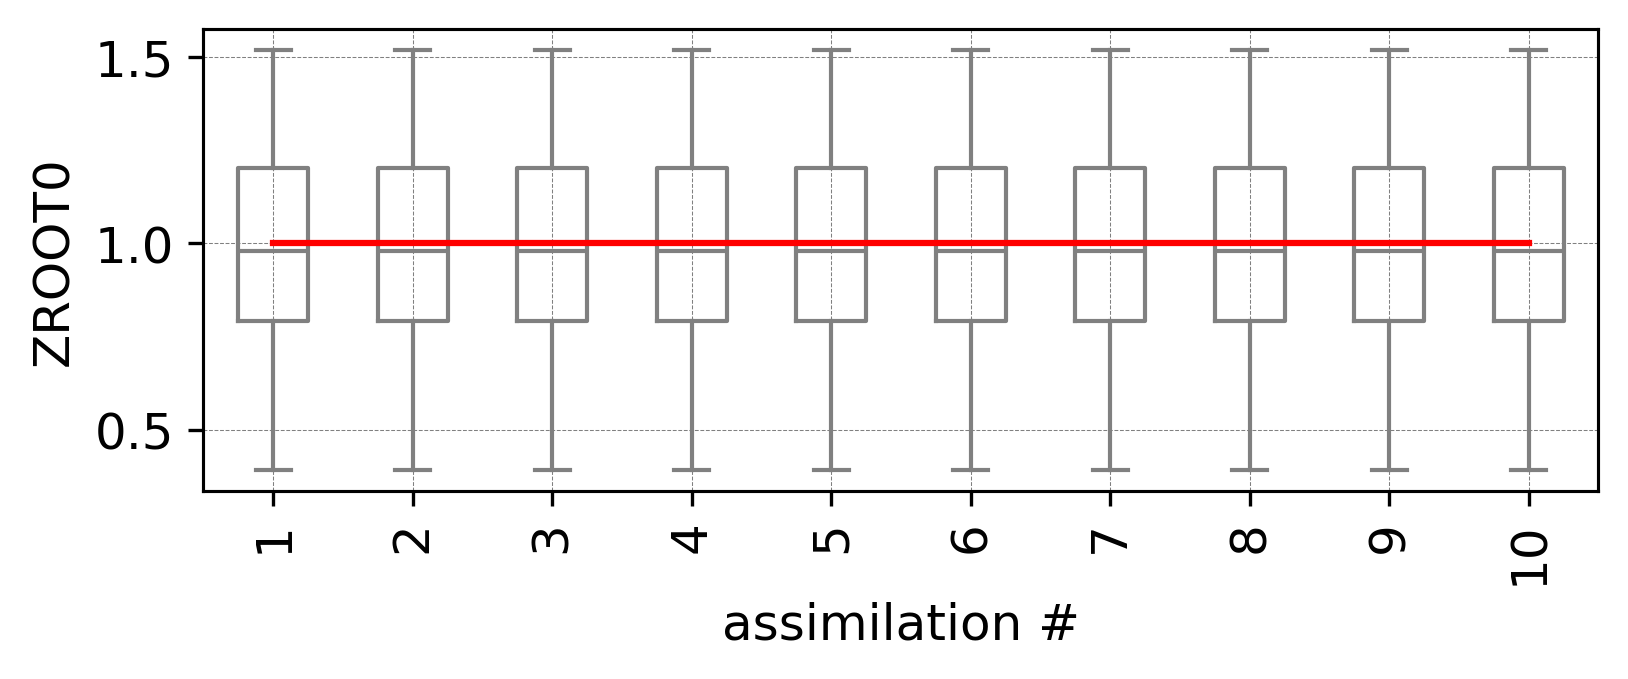
\includegraphics[width=0.75\linewidth]{files/meshLi_withoutDA_ZRO-ba31c6c59b620a6e618131fdaa21284b.png}
\caption[]{meshLi\_withoutDA\_ZROOT\_WITH\_UPDATE\_ZROOT}
\label{meshLi_withoutDA_ZROOT_WITH_UPDATE_ZROOT}
\end{figure}

\begin{figure}[!htbp]
\centering
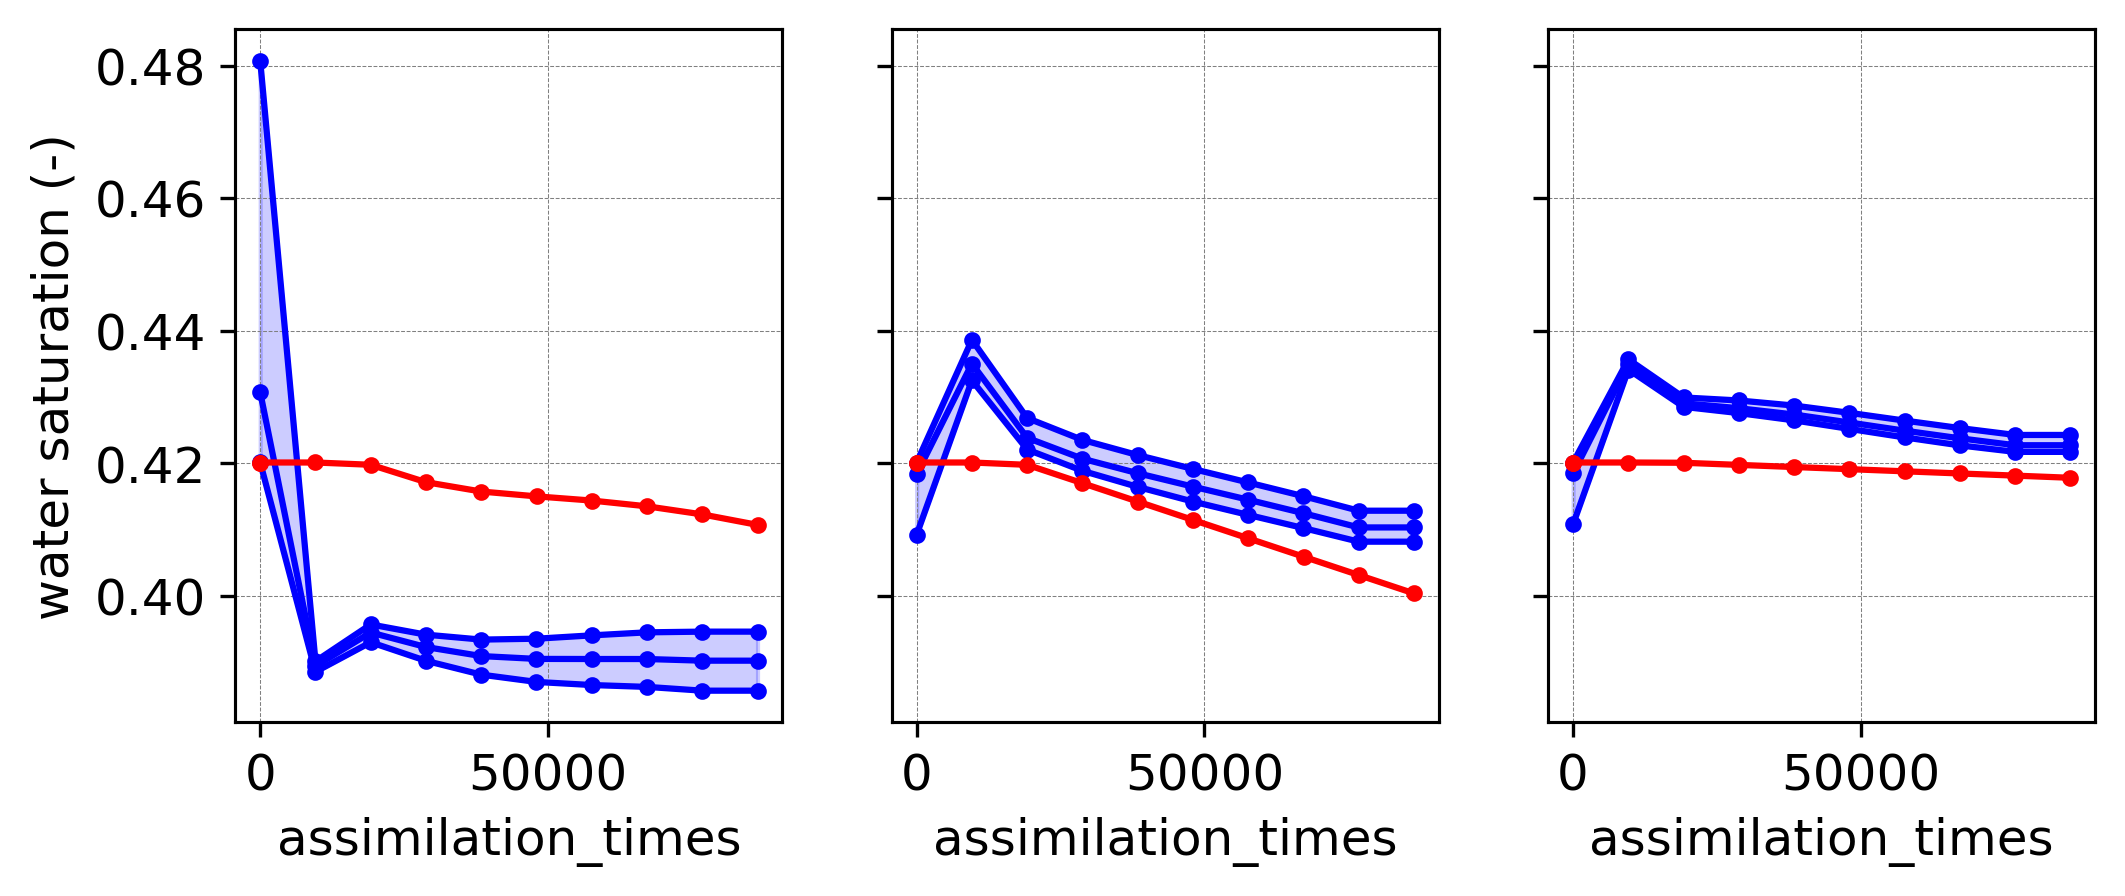
\includegraphics[width=0.75\linewidth]{files/meshLi_withDA_ZROOT_-9dcd843c7ecc77571709f13912526f64.png}
\caption[]{meshLi\_withDA\_ZROOT\_WITH\_UPDATE\_sw}
\label{meshLi_withDA_ZROOT_WITH_UPDATE_sw}
\end{figure}

\begin{figure}[!htbp]
\centering
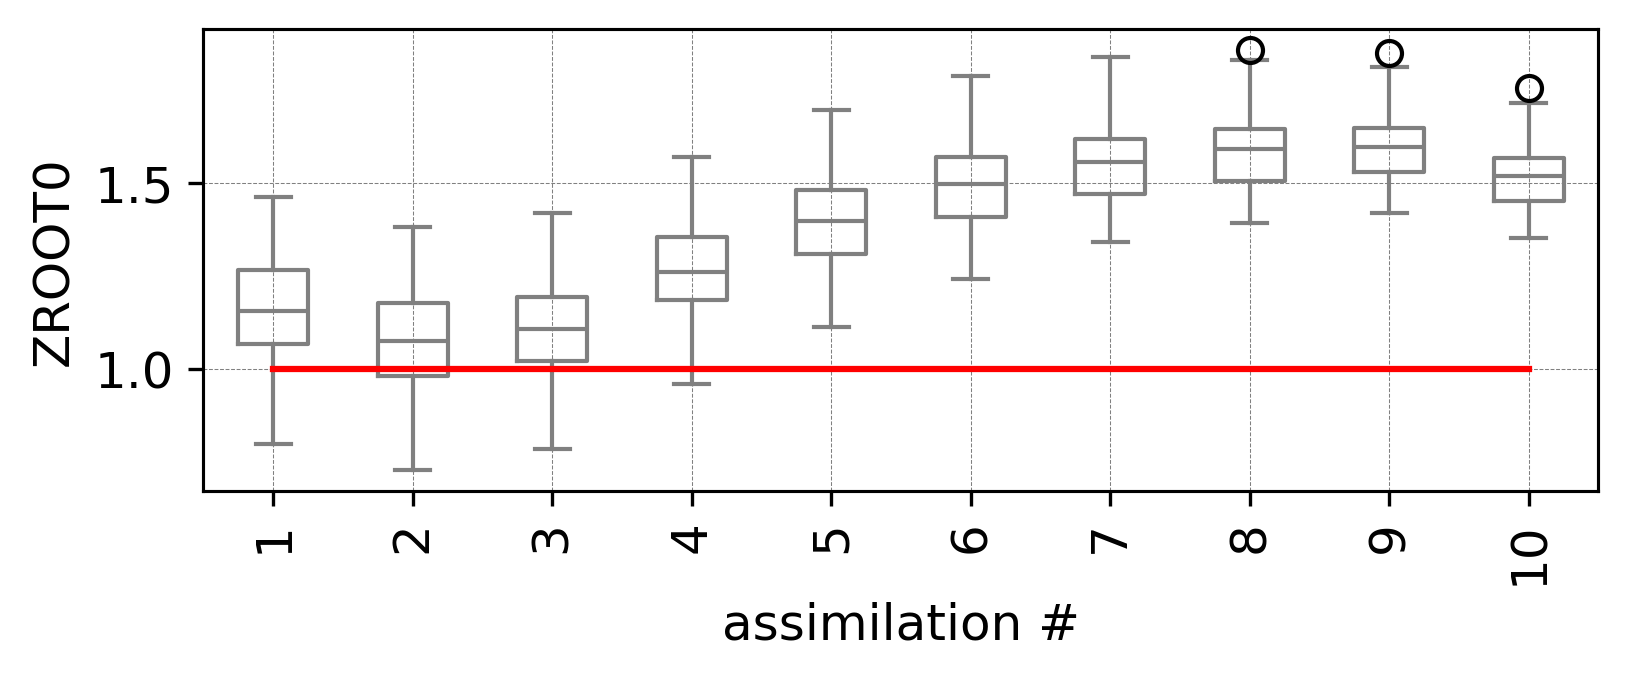
\includegraphics[width=0.75\linewidth]{files/meshLi_withDA_ZROOT_-841c61080a979f5d7317d36b67fbe998.png}
\caption[]{meshLi\_withDA\_ZROOT\_WITH\_UPDATE\_ZROOT}
\label{SMC_withoutDA_icsw}
\end{figure}

\section{Actual ET}

\section{Model 1: variable spatial ZROOT depth}

\textbf{True State Generation}
The true state of soil moisture is generated by running a hydrological model with \textbf{known parameters and forcing data} over a 24-hour period. This true state serves as the synthetic reality for the experiment.

\begin{figure}[!htbp]
\centering
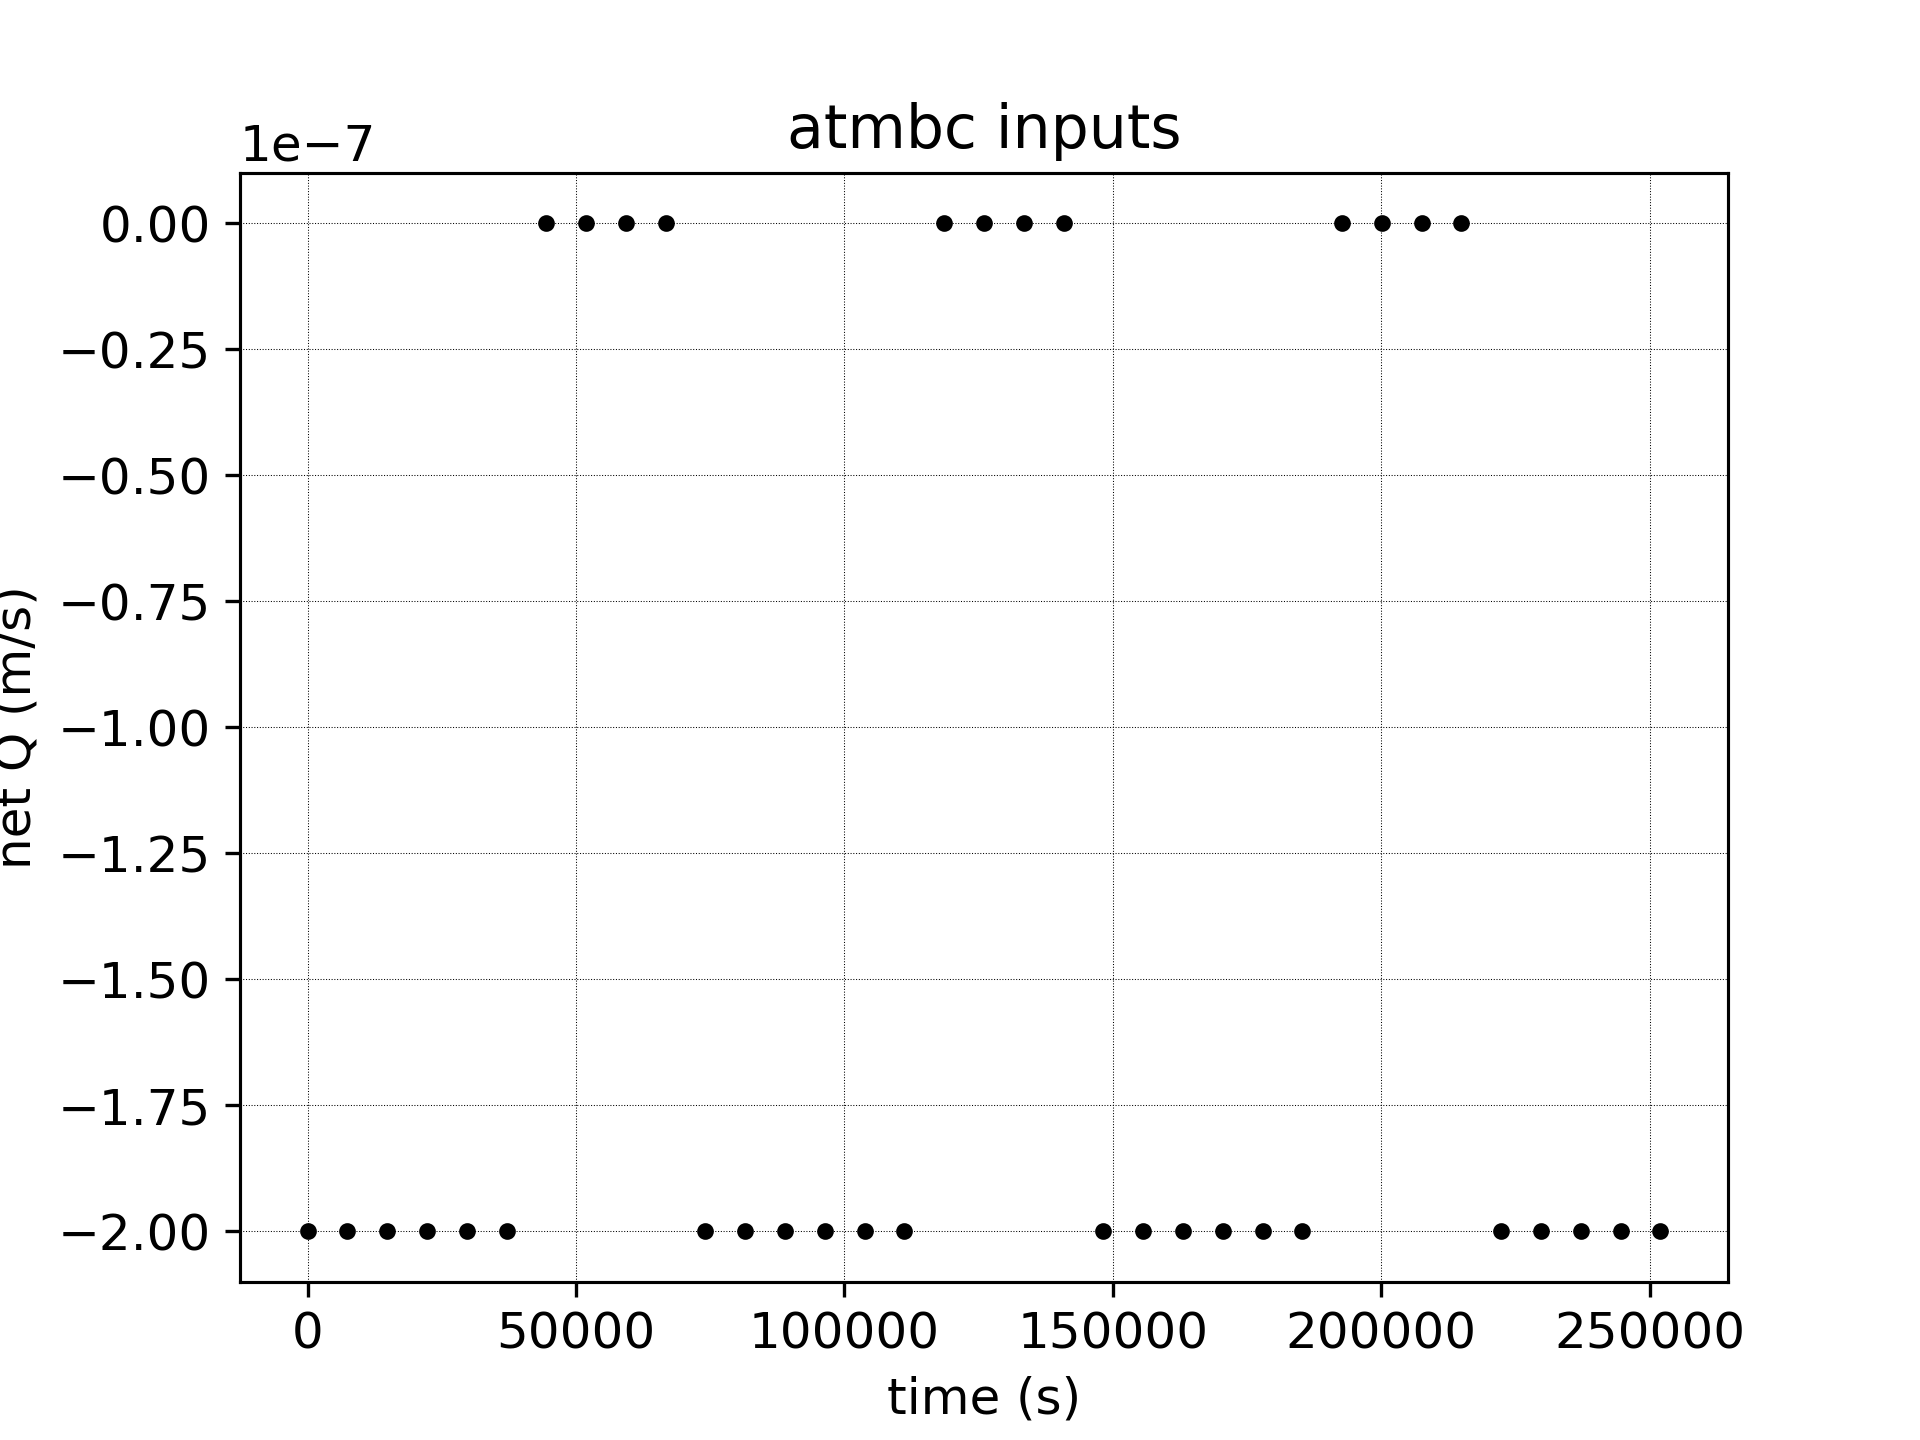
\includegraphics[width=0.75\linewidth]{files/atmbc-312192448aa4c0a1e57cb587d79a2dbc.png}
\caption[]{True-state-atmbc}
\label{true-state-atmbc}
\end{figure}

\begin{figure}[!htbp]
\centering
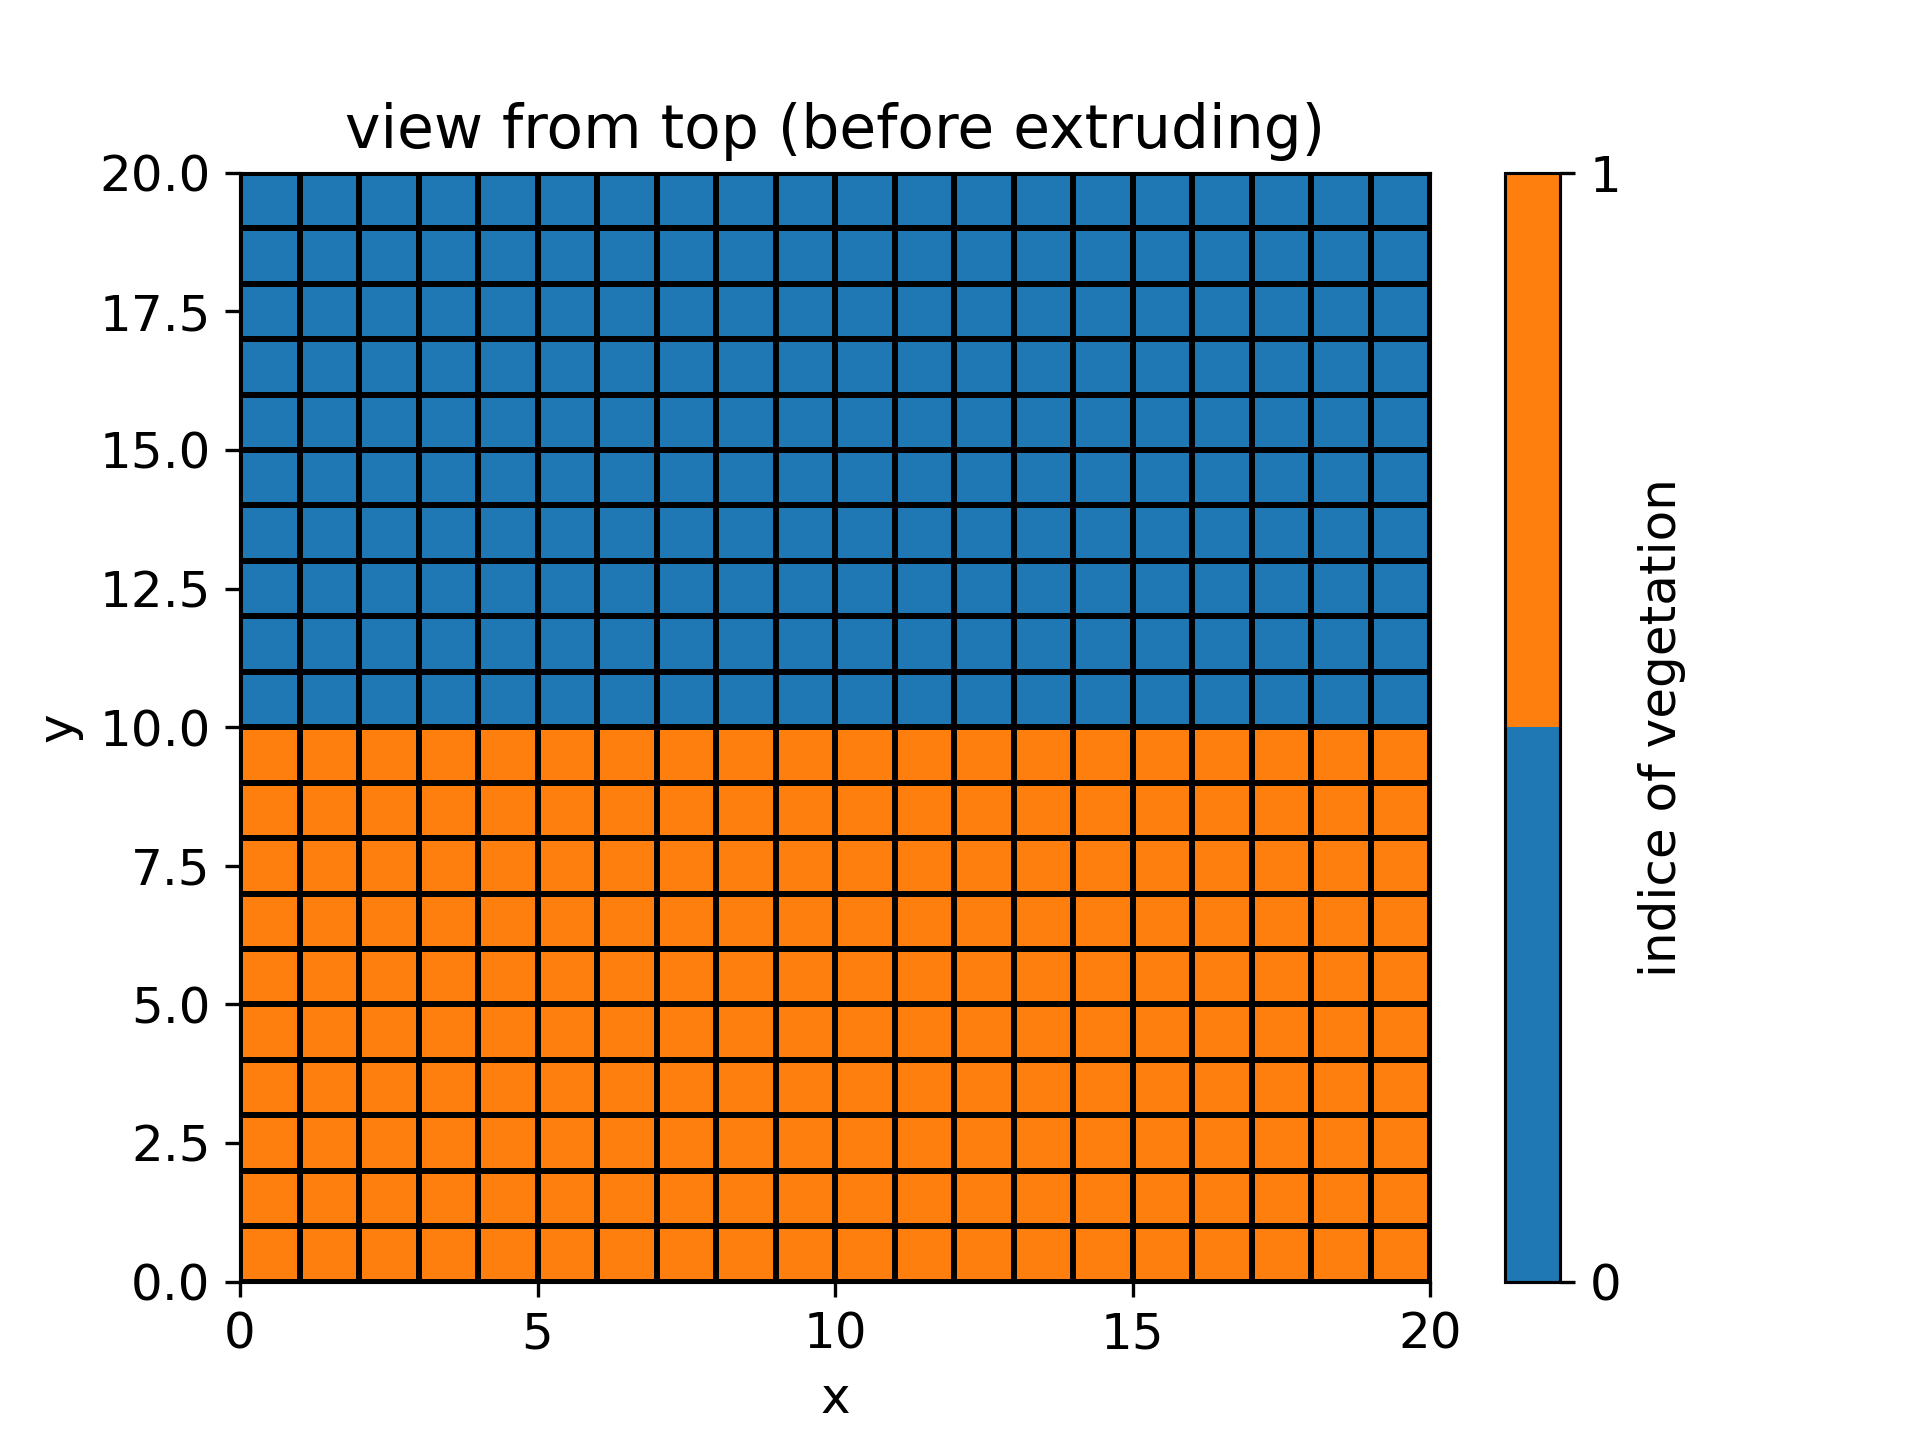
\includegraphics[width=0.75\linewidth]{files/ZROOT_spatially_from-7ecc3d61ffe164d15040448f6d1d09eb.png}
\caption[]{True-state-ZROOT\_spatially\_from\_weillroot\_map}
\label{true-state-ZROOT_spatially_from_weillroot_map}
\end{figure}

\begin{figure}[!htbp]
\centering
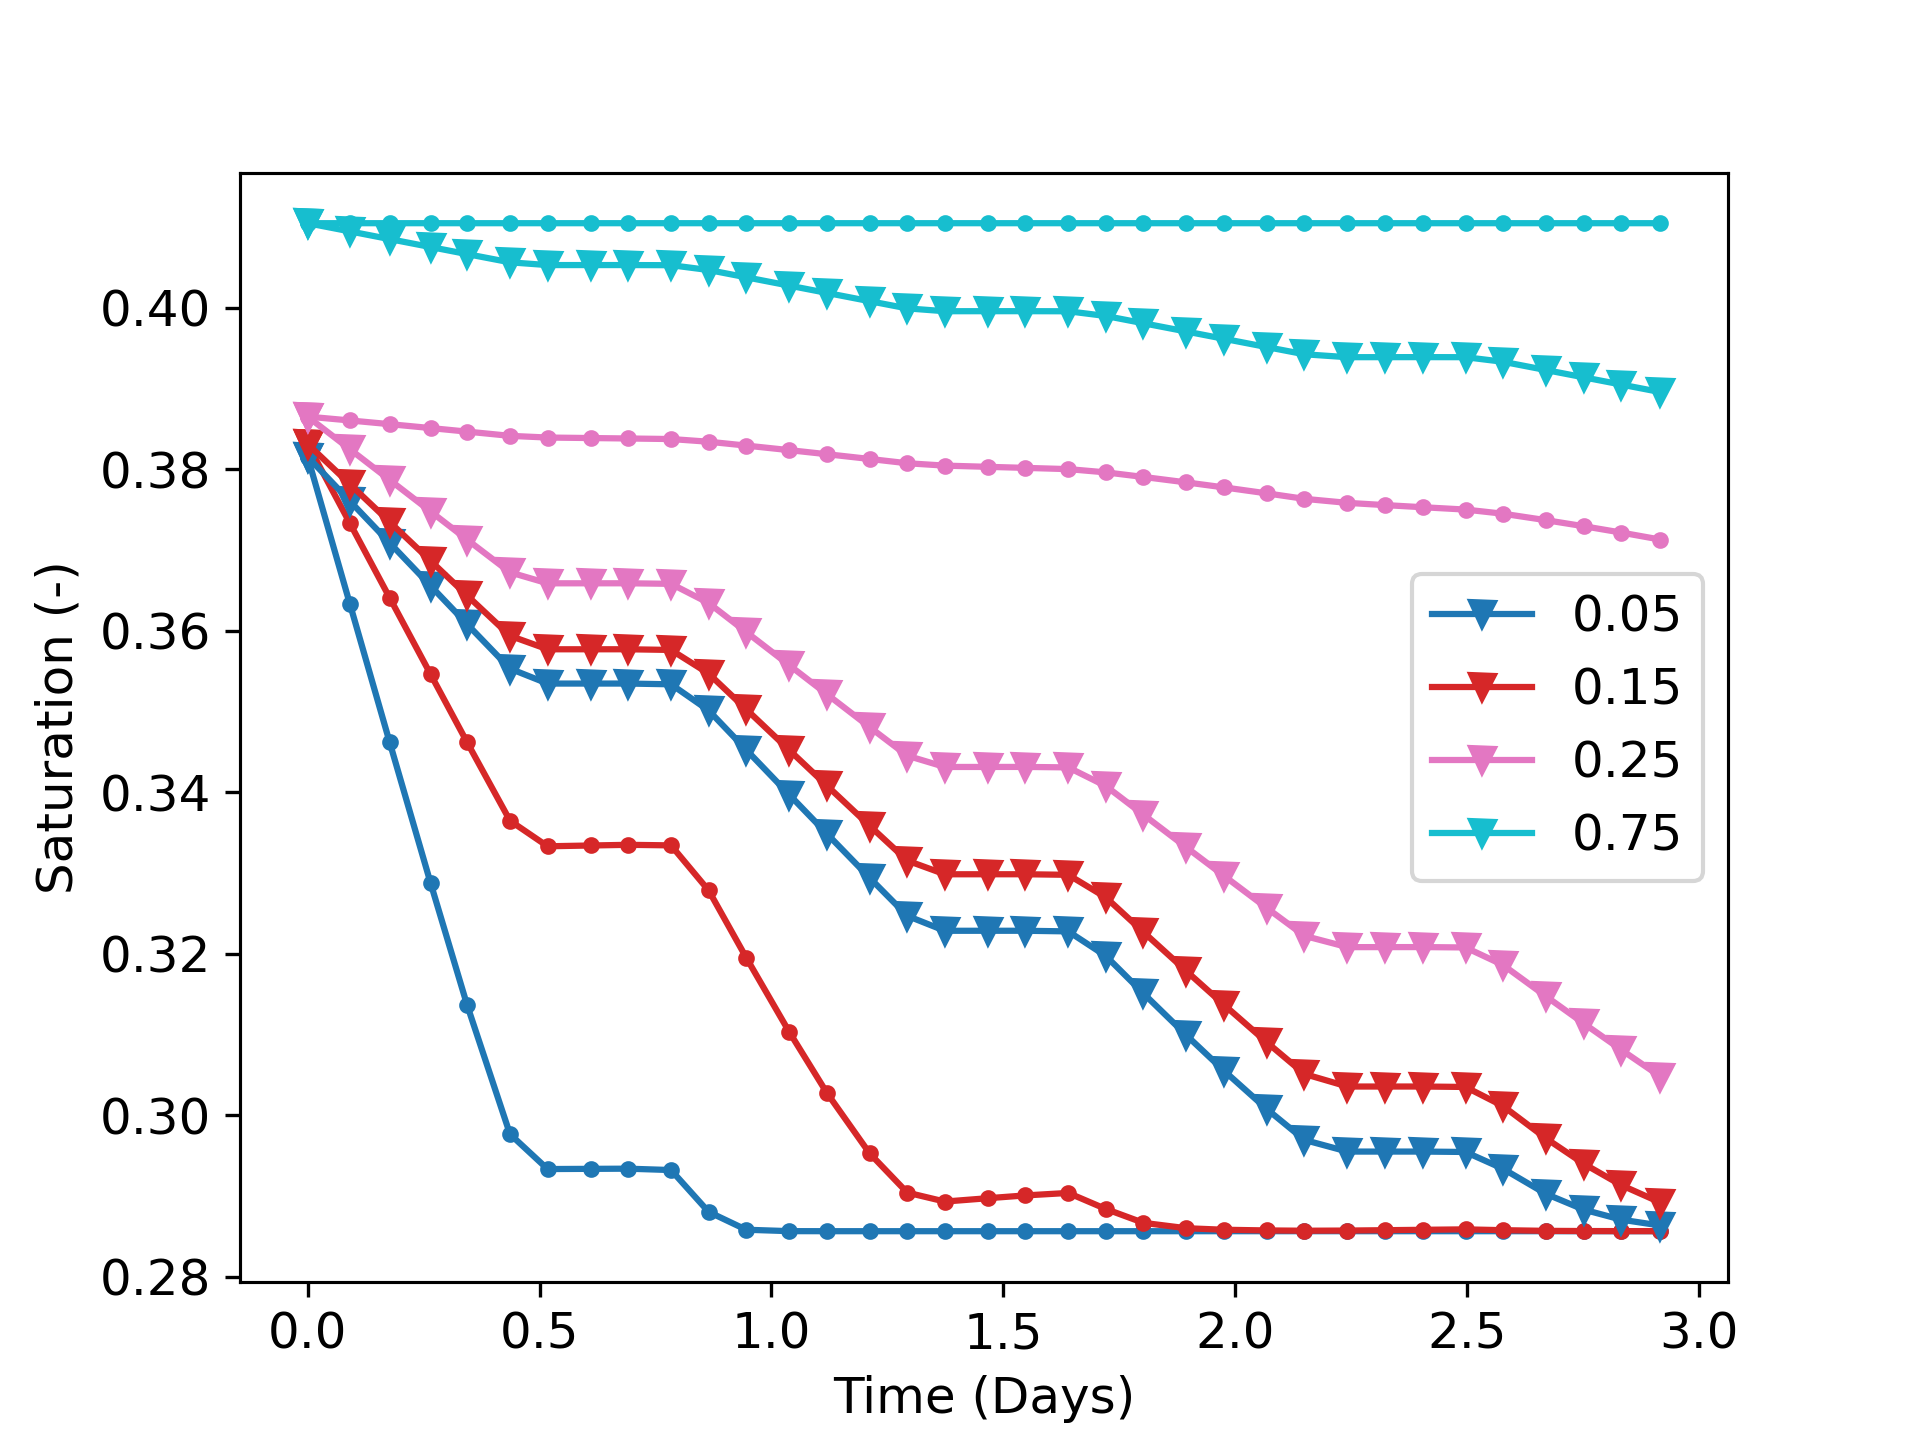
\includegraphics[width=0.75\linewidth]{files/ZROOT_spatially_from-0ce95c7463d4c2fe8a10cb04bfa38e8c.png}
\caption[]{True-state-ZROOT\_spatially\_from\_weillsw}
\label{true-state-ZROOT_spatially_from_weillsw}
\end{figure}

\begin{figure}[!htbp]
\centering
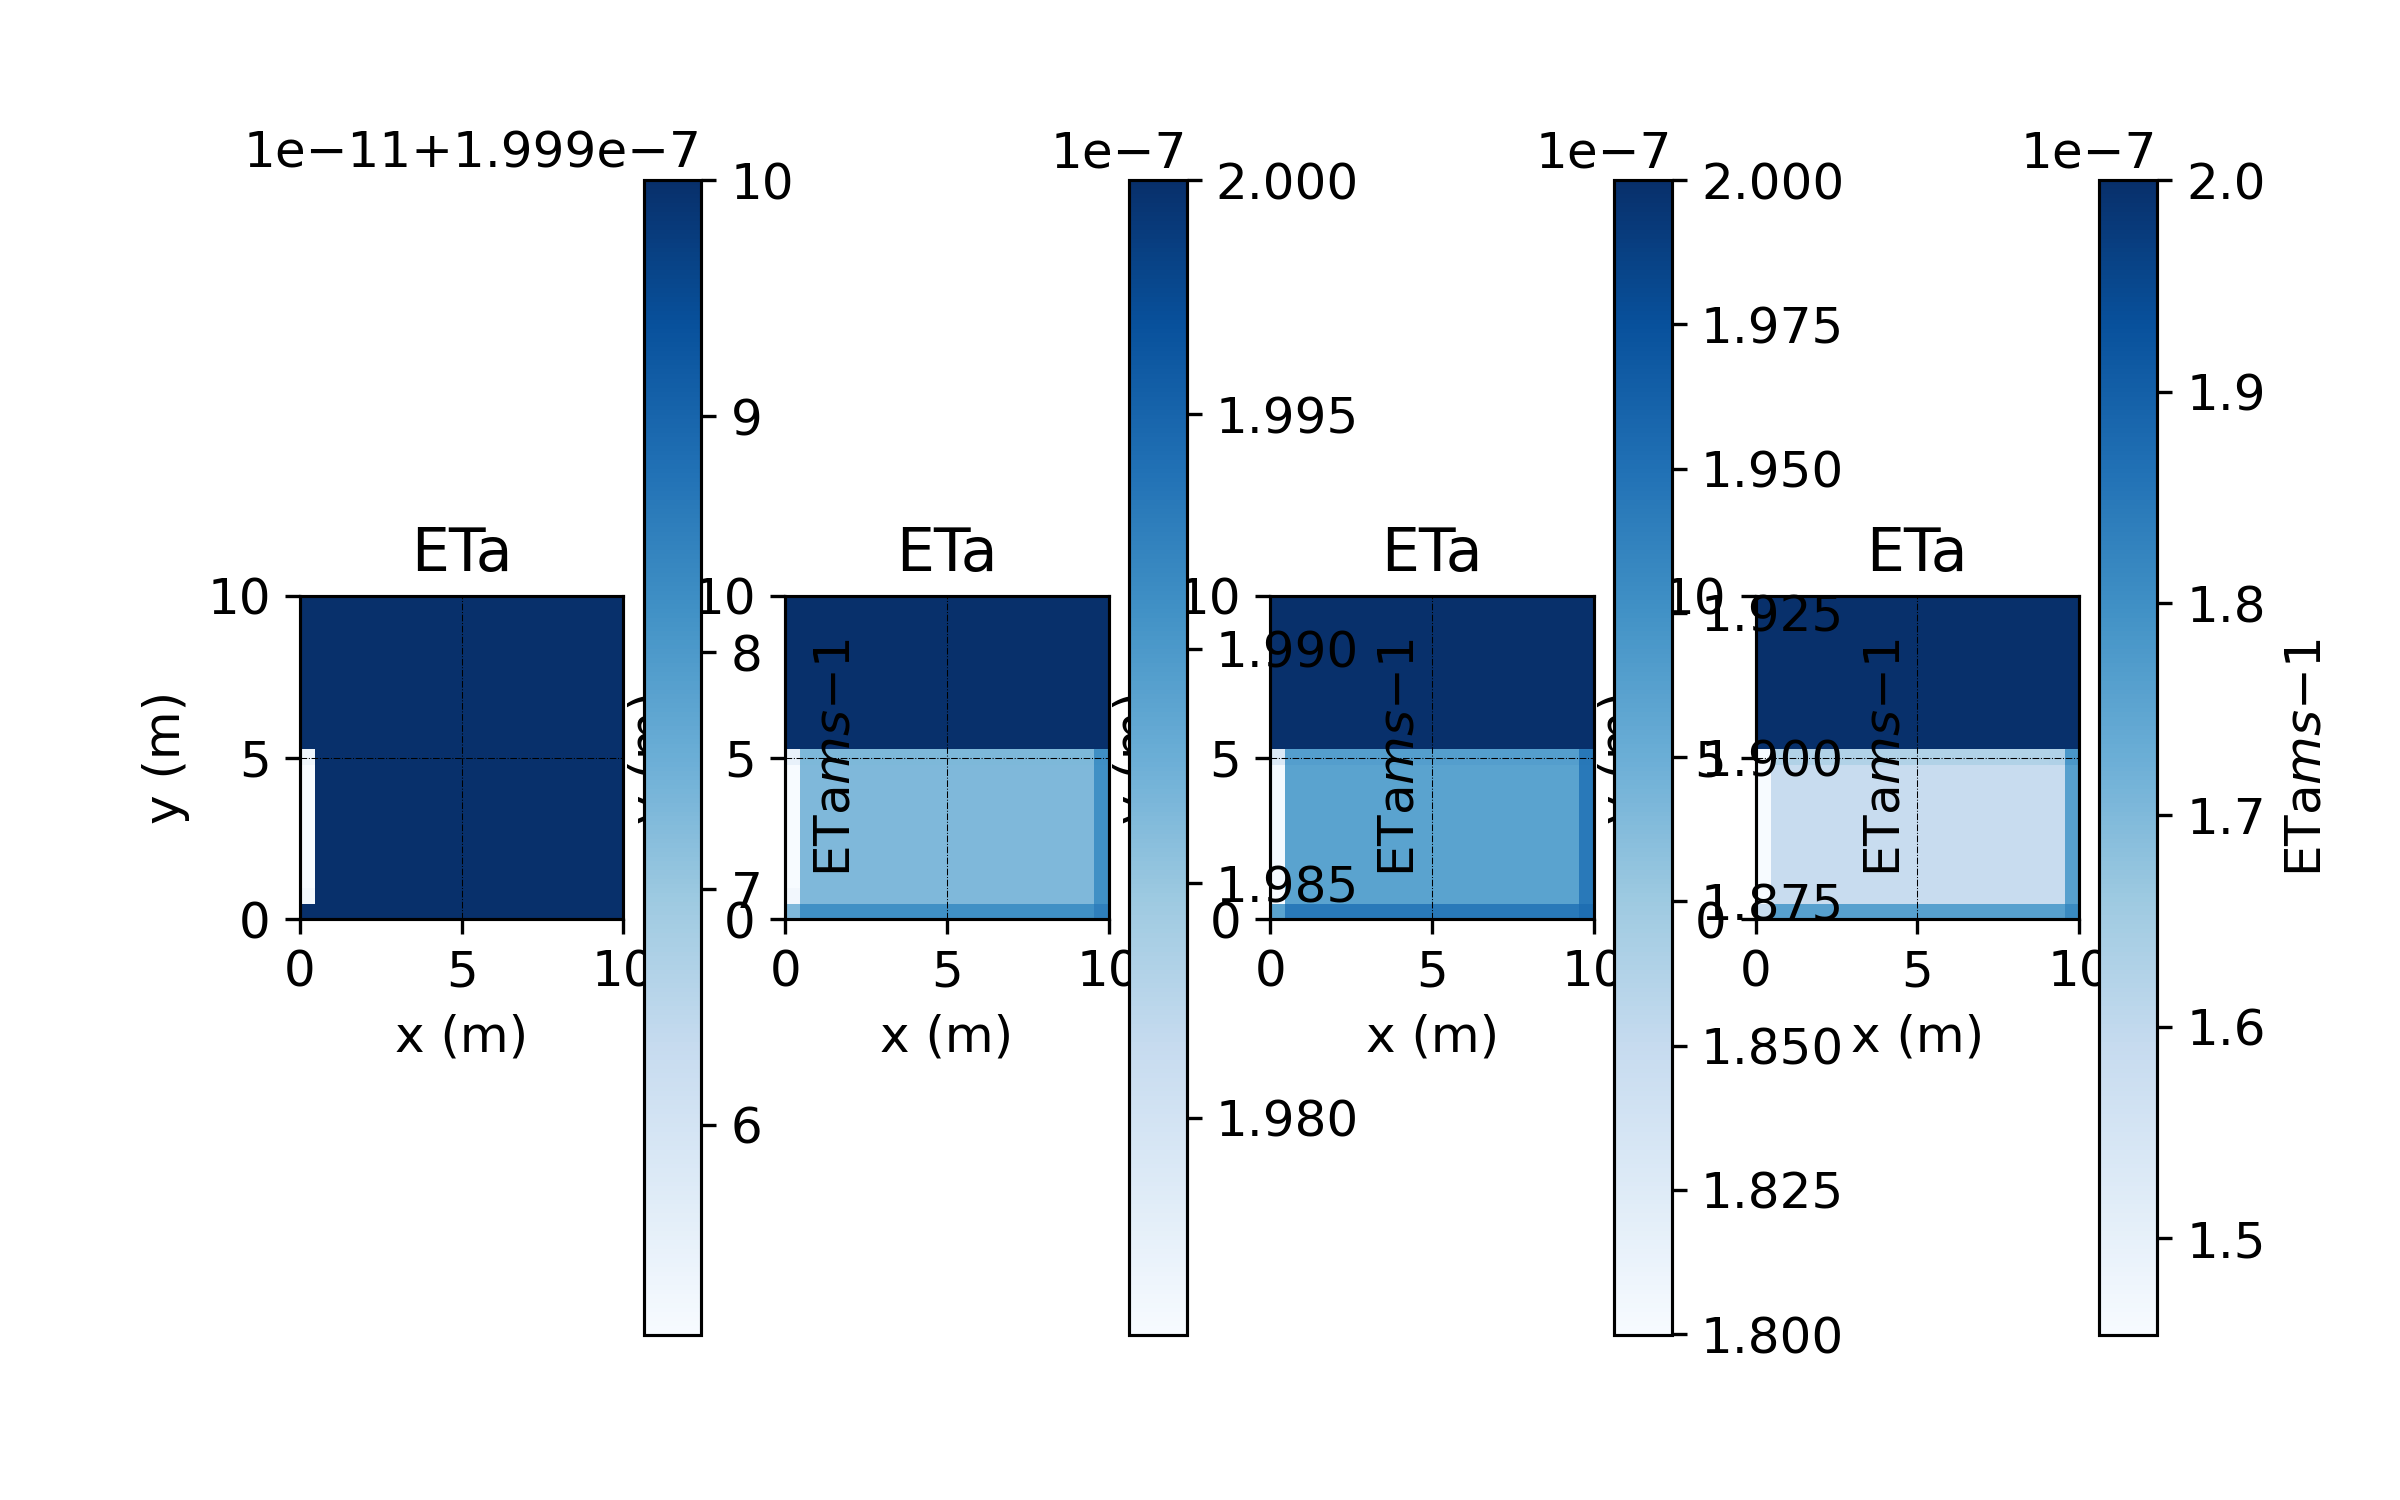
\includegraphics[width=0.75\linewidth]{files/ZROOT_spatially_from-e0b830dc4e6efc439d94598aafc098b2.png}
\caption[]{ZROOT\_spatially\_from\_weillspatialET}
\label{ZROOT_spatially_from_weillspatialET}
\end{figure}

\begin{figure}[!htbp]
\centering
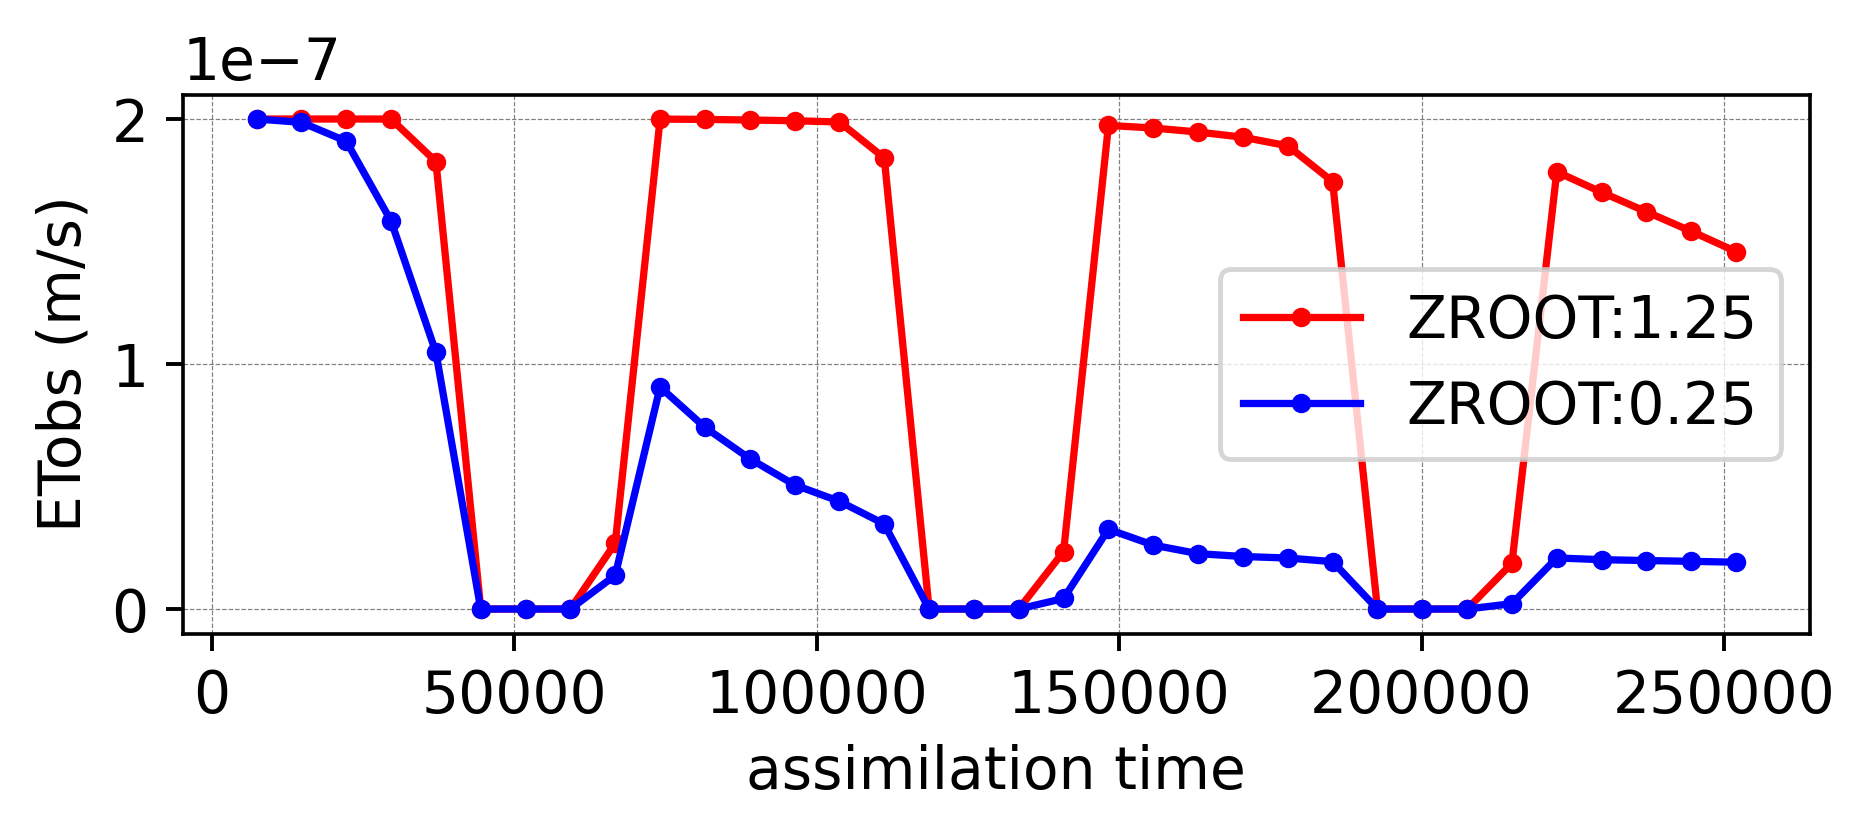
\includegraphics[width=0.75\linewidth]{files/atmbc_pernodes-4453e76d81b2f73f09dec96e9257c4c1.png}
\caption[]{atmbc\_pernodes}
\label{atmbc_pernodes}
\end{figure}

\textbf{Perturbed Initial State}
A new simulation of the hydrological model is initiated with perturbed initial conditions and/or parameters. This represents the model's initial guess, which deviates from the true state.

\begin{figure}[!htbp]
\centering
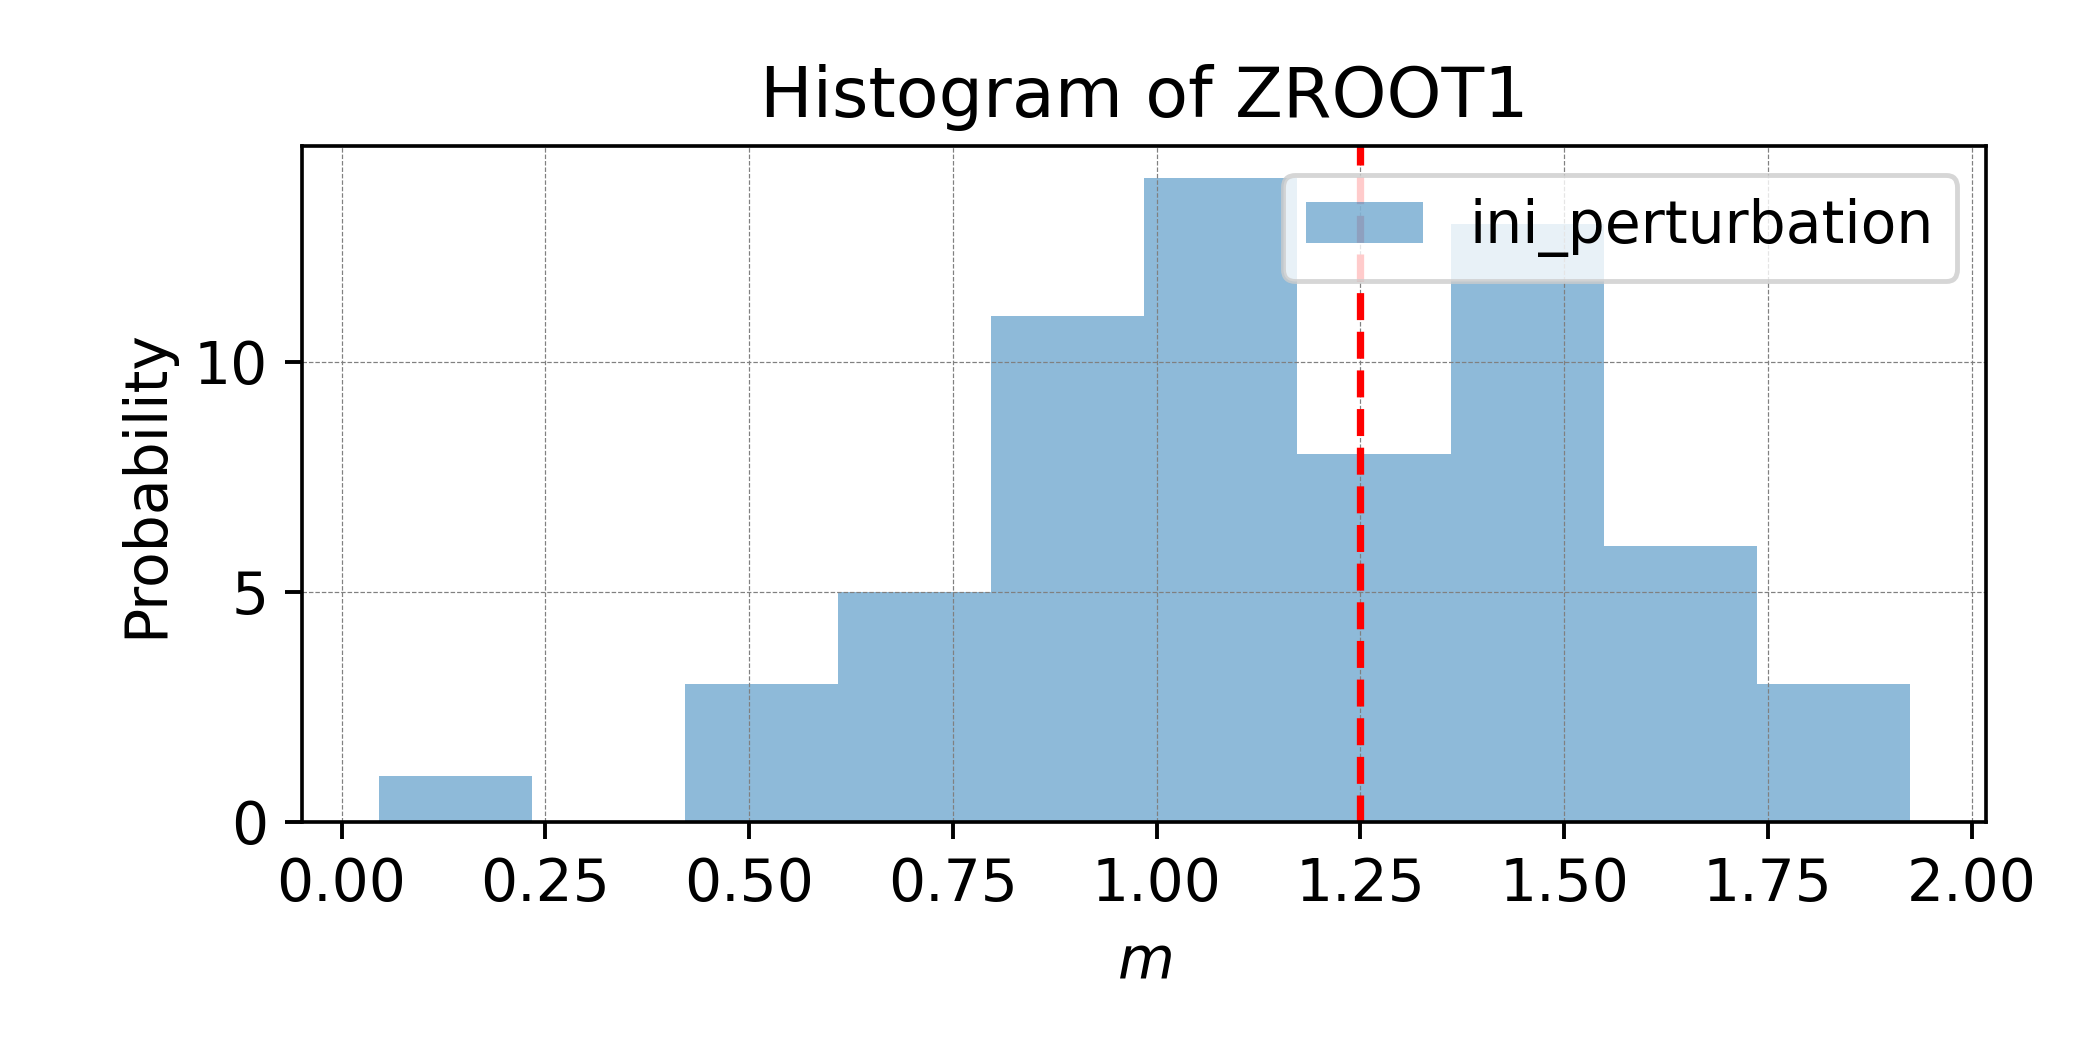
\includegraphics[width=0.75\linewidth]{files/DA_ET_0ZROOT1-5513eabe5380a9280afae0dfbaa2f6e2.png}
\caption[]{DA\_ET\_0ZROOT1}
\label{DA_ET_0ZROOT1}
\end{figure}

\begin{figure}[!htbp]
\centering
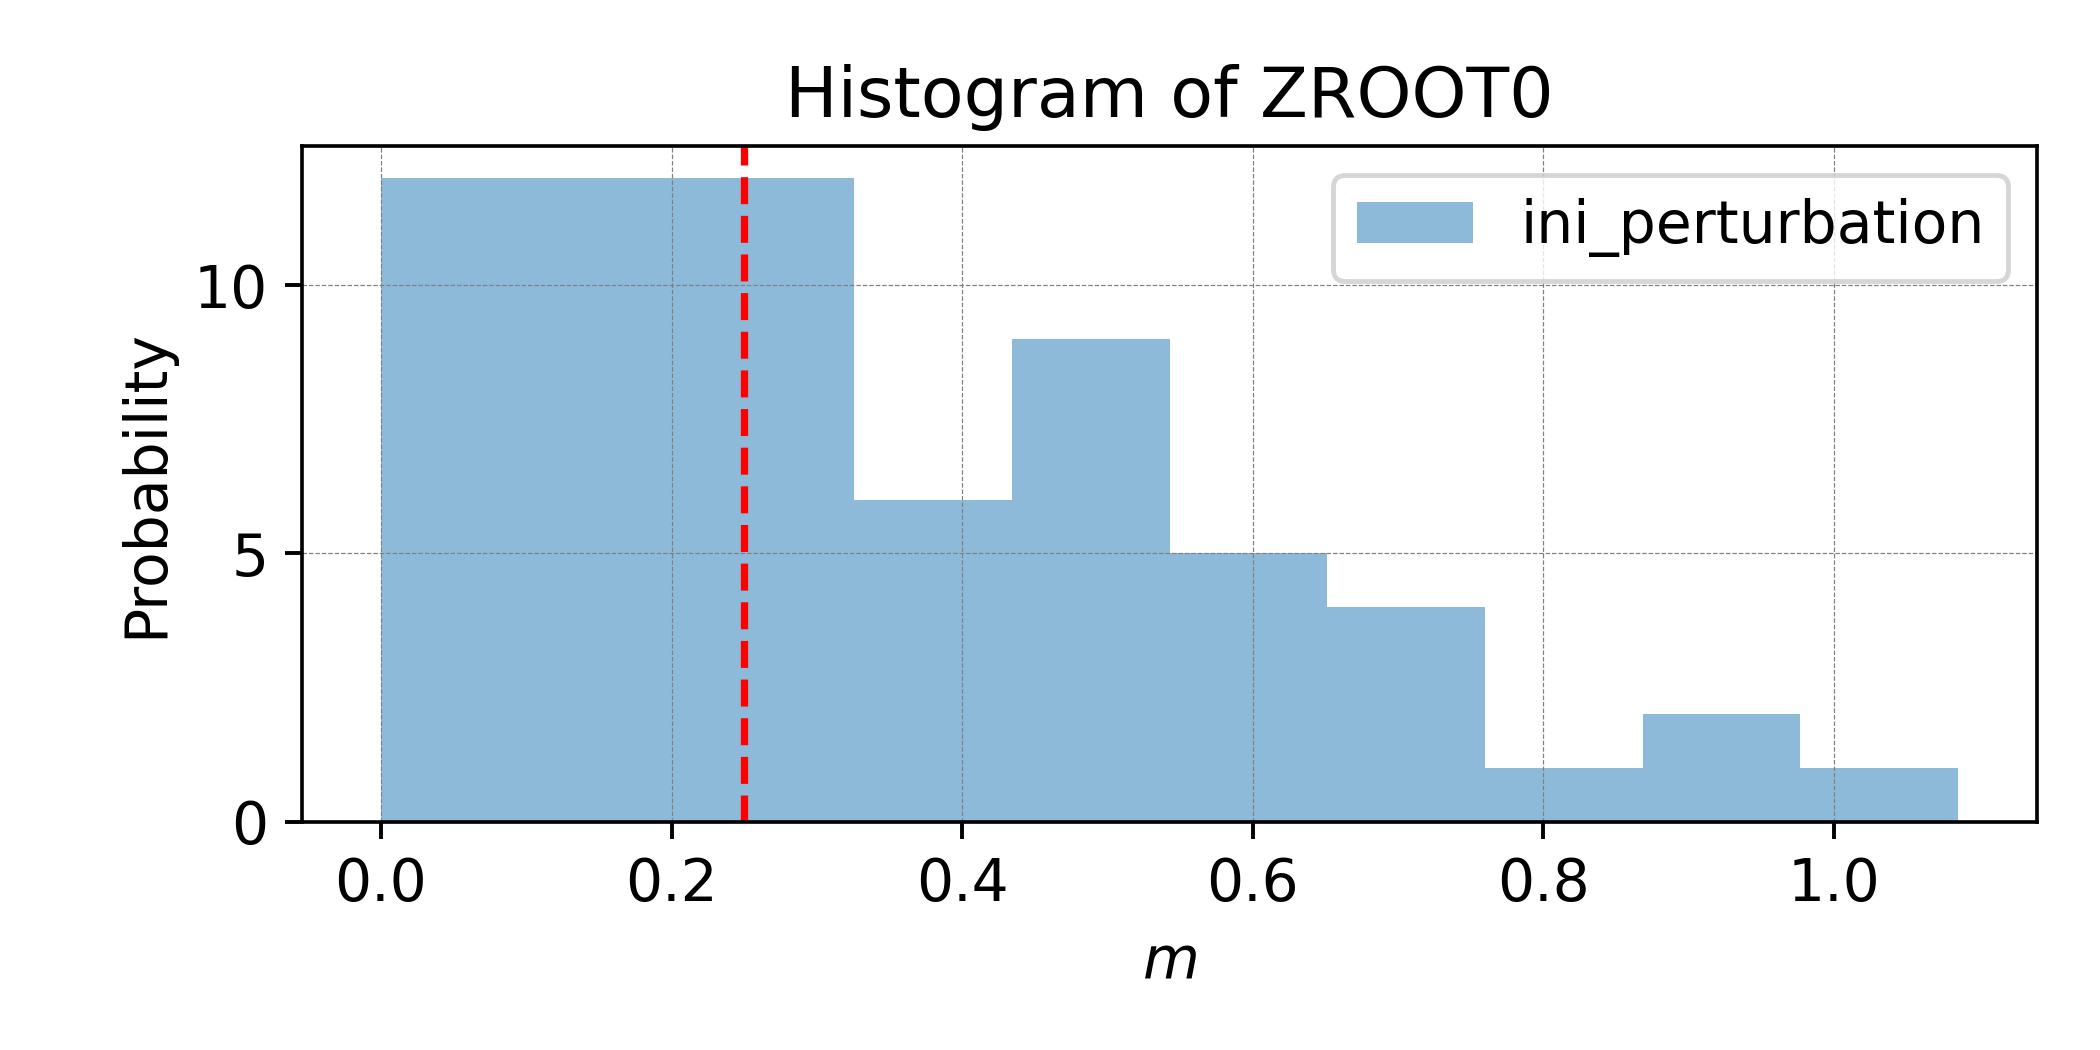
\includegraphics[width=0.75\linewidth]{files/DA_ET_0ZROOT0-17556b113c91aeb53d1c9e920273c790.png}
\caption[]{DA\_ET\_0ZROOT0}
\label{DA_ET_0ZROOT0}
\end{figure}

\textbf{Data Assimilation}
The synthetic observations are assimilated into the hydrological model using the Ensemble Kalman Filter (EnKF) method. This process updates the model state to better match the observations.

\textbf{Analysis and Evaluation}
The performance of the data assimilation is evaluated by comparing the assimilated model state with the true state. Metrics such as root mean square error (RMSE) are used to quantify the accuracy of the assimilation.

\subsection{Water table perturbations}

\subsection{Root depth perturbations and update}

\subsubsection{Without Update}

\begin{figure}[!htbp]
\centering
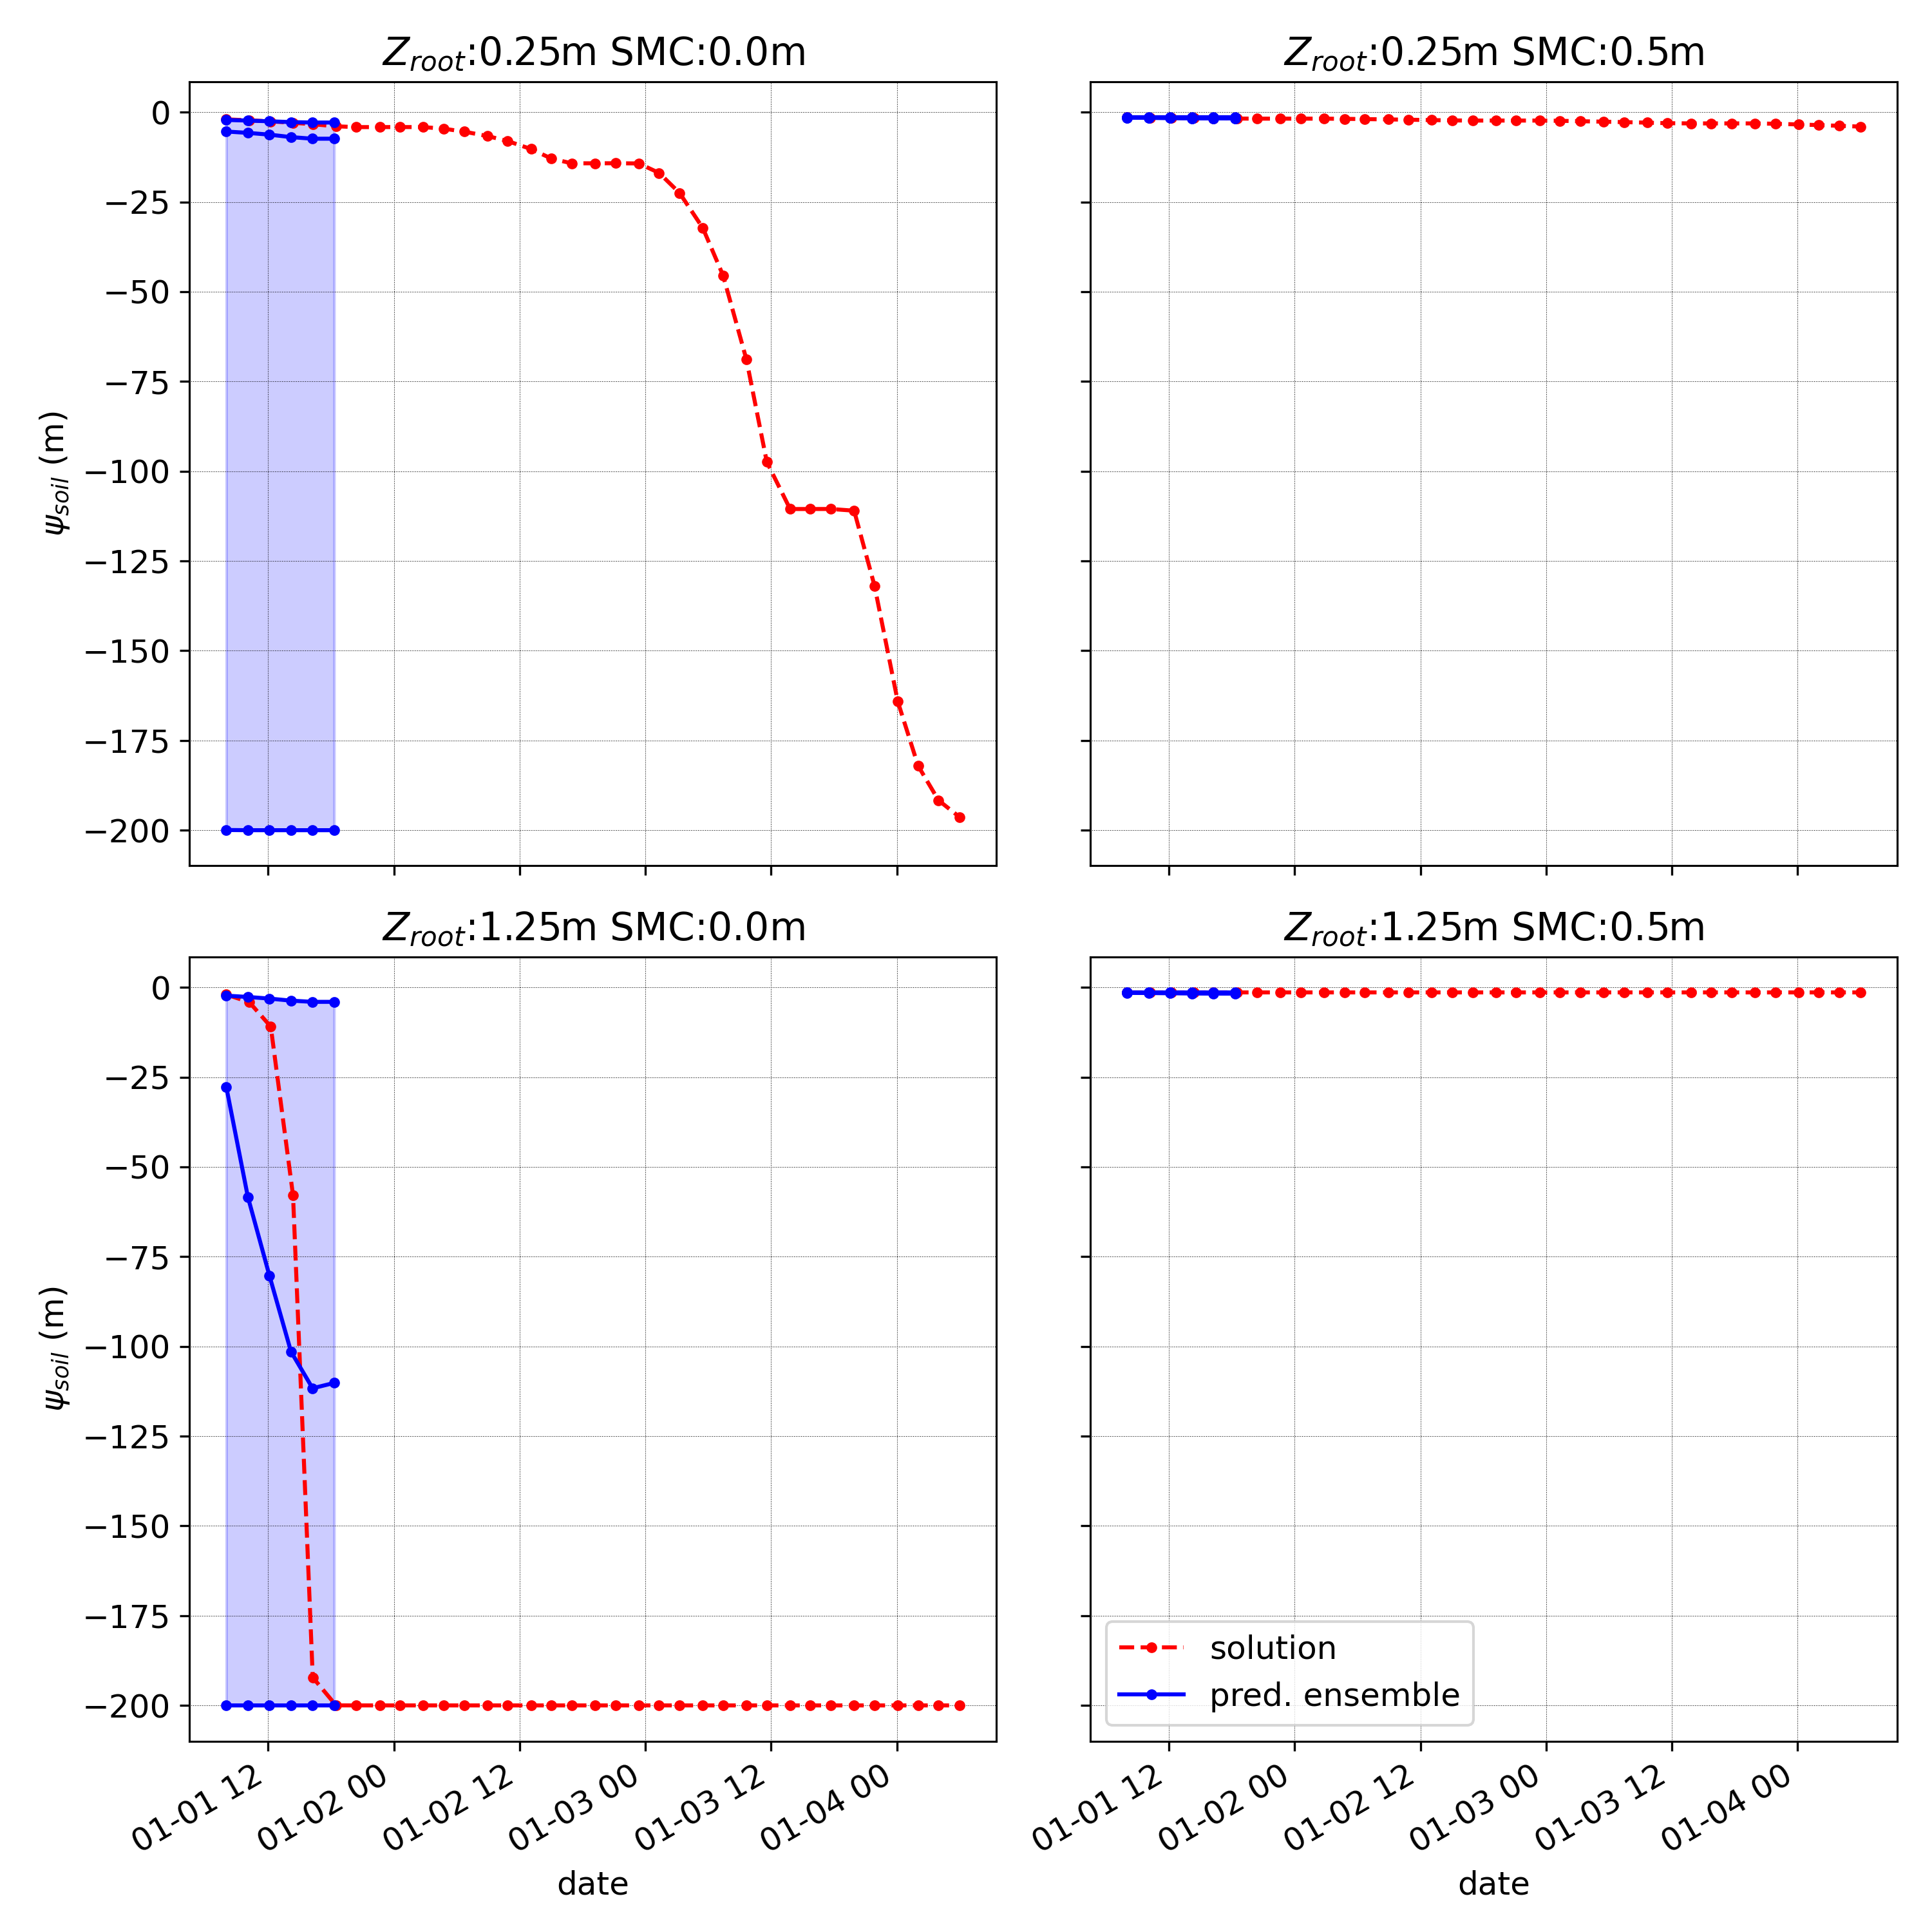
\includegraphics[width=0.75\linewidth]{files/states_dyn_psi-68368e11811a97694a714da212117983.png}
\caption[]{states\_dyn\_psi}
\label{states_dyn_psi}
\end{figure}

\begin{figure}[!htbp]
\centering
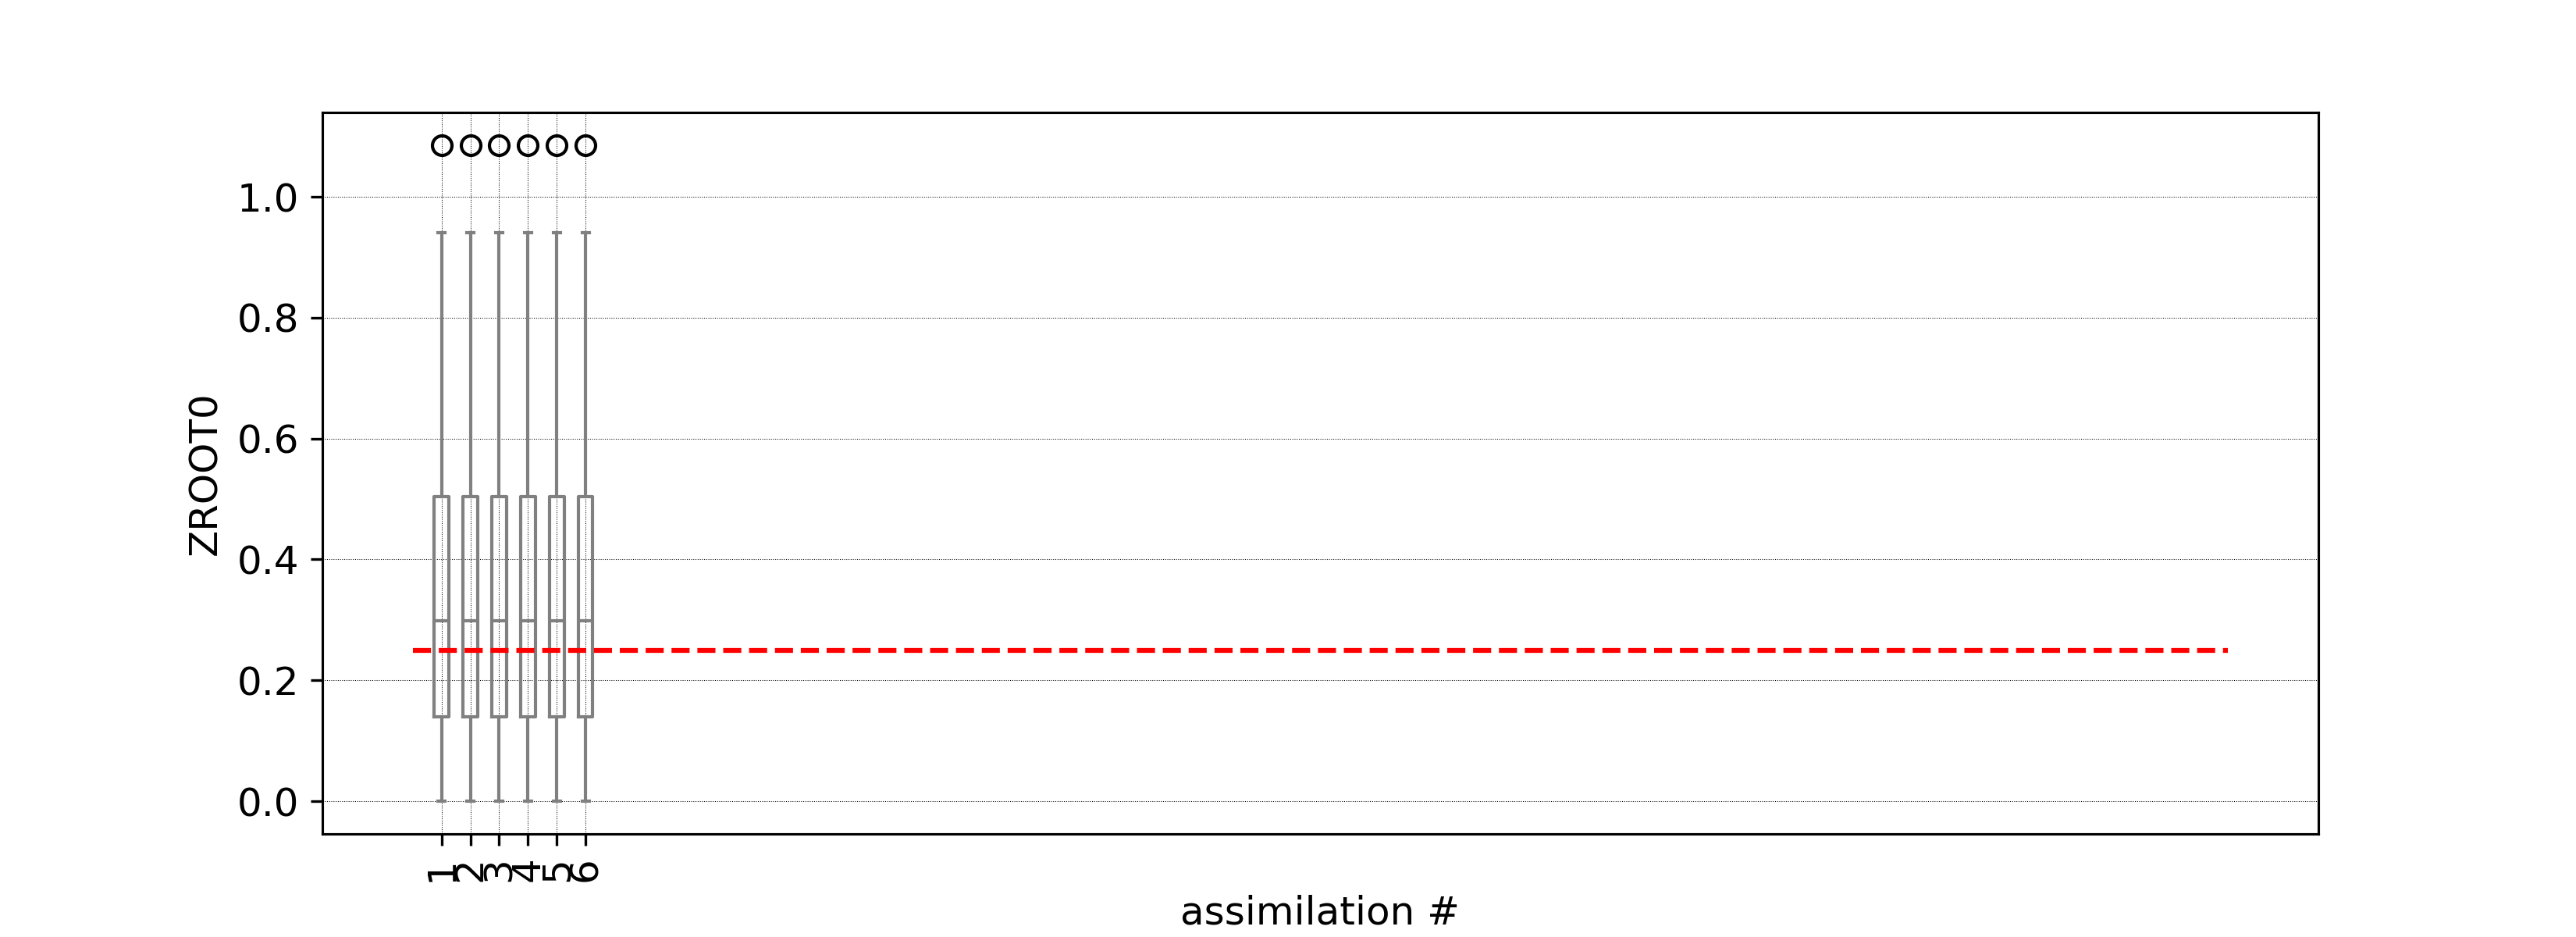
\includegraphics[width=0.75\linewidth]{files/ZROOT0-7a4a9fa8cfc5ad5d17d9cf18aec10168.png}
\caption[]{ZROOT0}
\label{ZROOT0}
\end{figure}

\begin{figure}[!htbp]
\centering
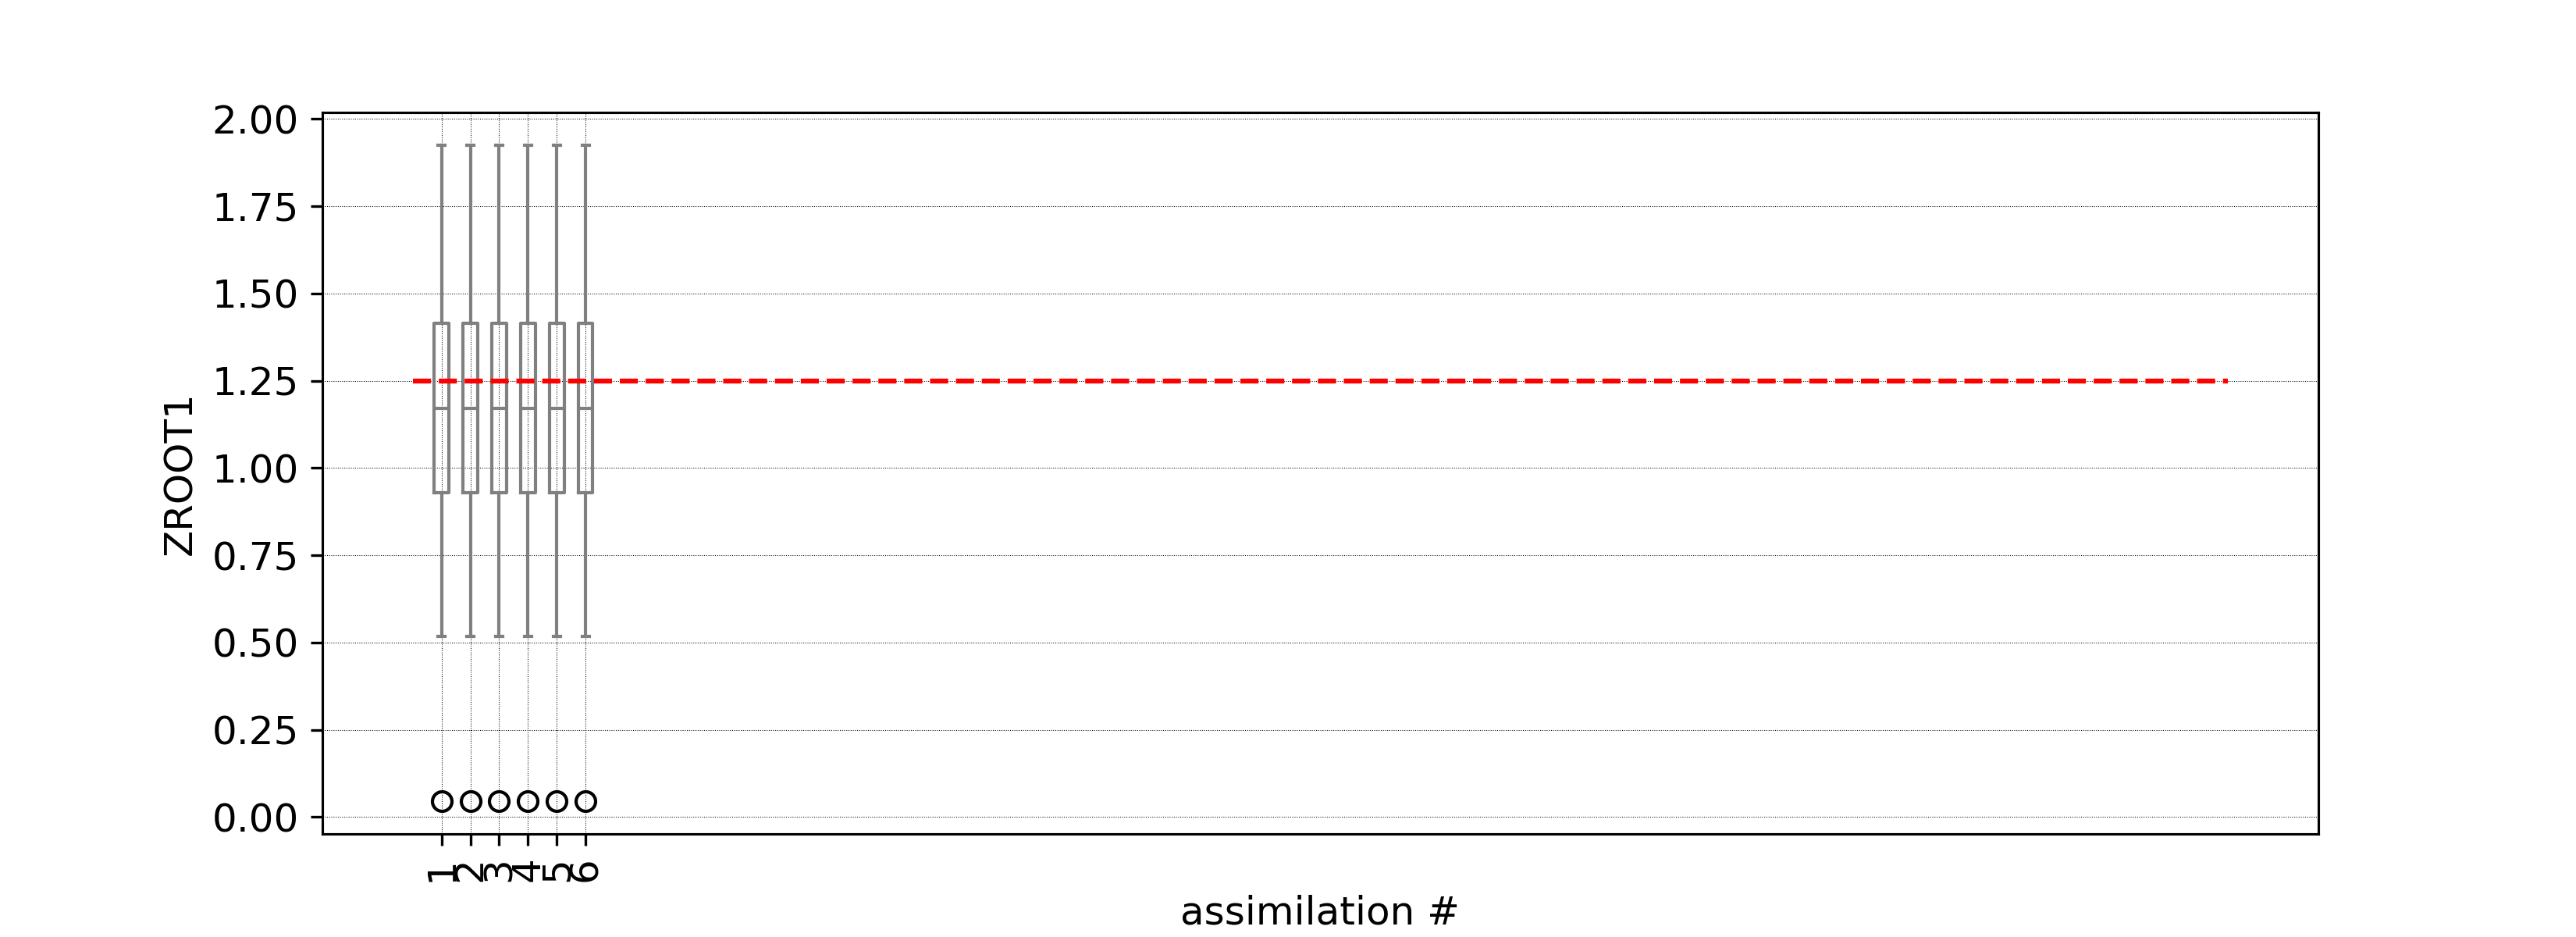
\includegraphics[width=0.75\linewidth]{files/ZROOT1-8b881abf587ac163f38dd9171ee4226a.png}
\caption[]{ZROOT0}
\label{ZROOT1}
\end{figure}

\subsubsection{With Update}

\begin{figure}[!htbp]
\centering
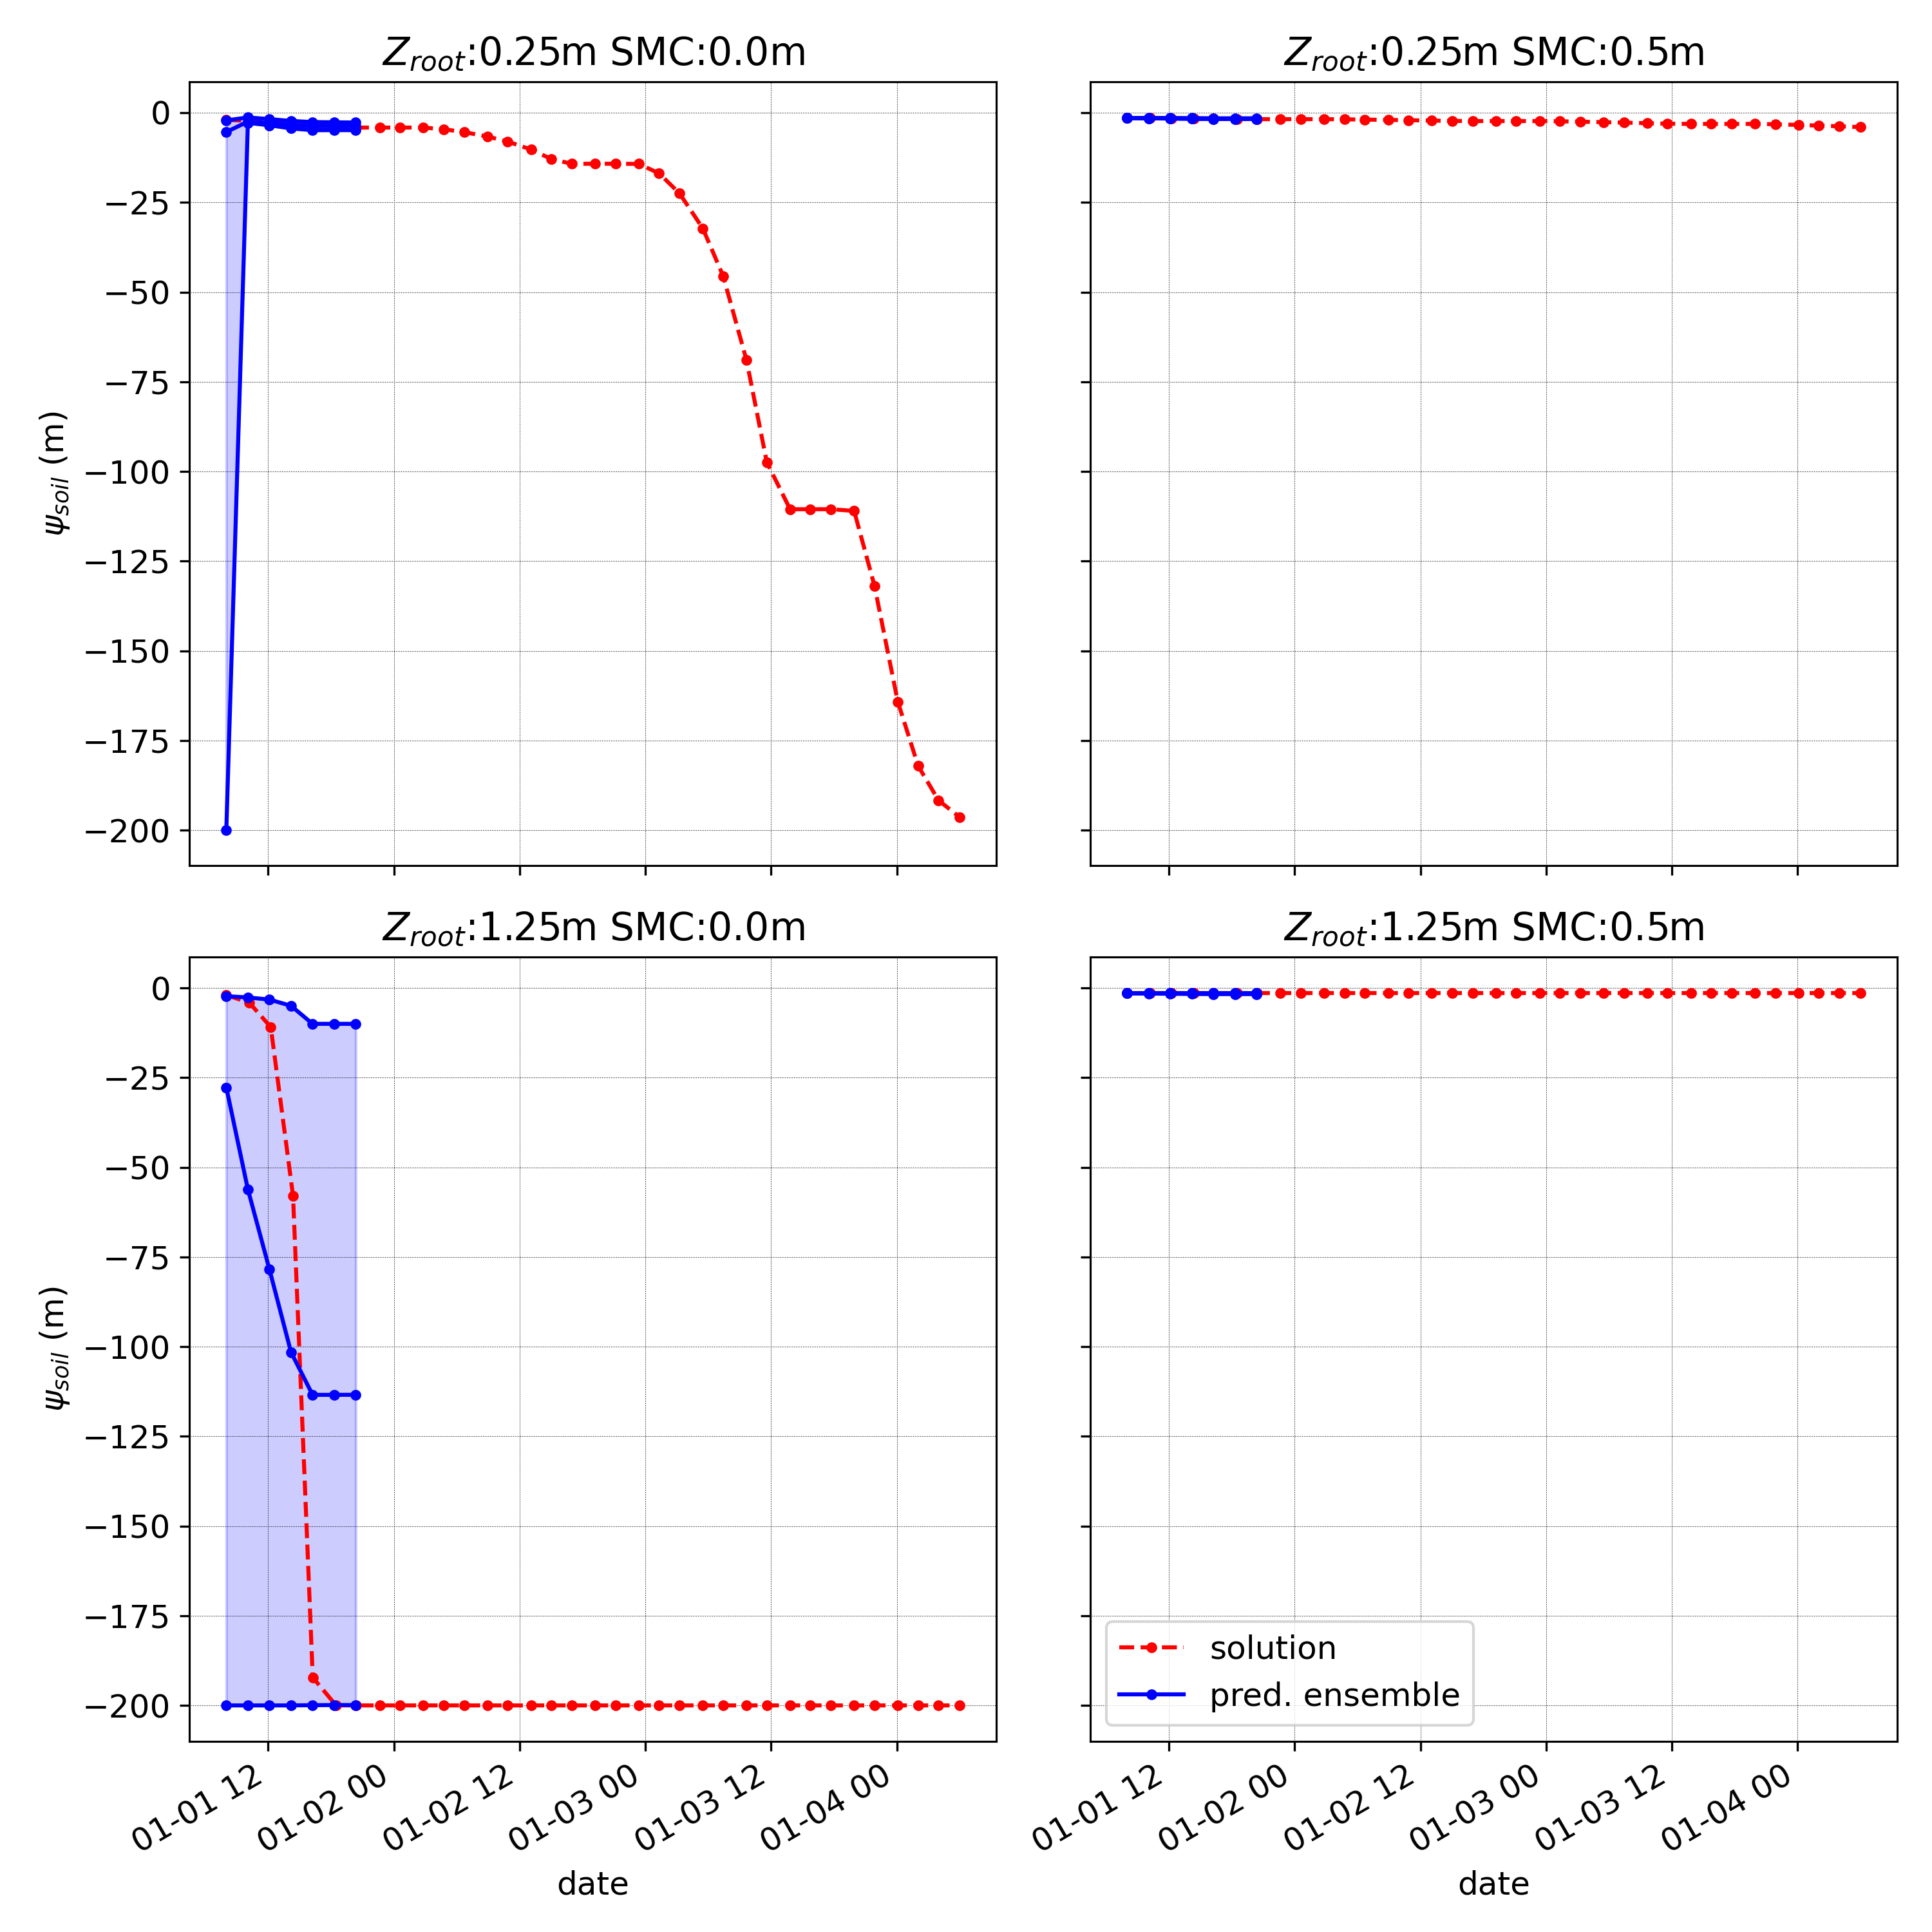
\includegraphics[width=0.75\linewidth]{files/states_dyn_psi-497f8e21155b6be00d8c34fca745139b.png}
\caption[]{states\_dyn\_psi}
\label{states_dyn_psi}
\end{figure}

\begin{figure}[!htbp]
\centering
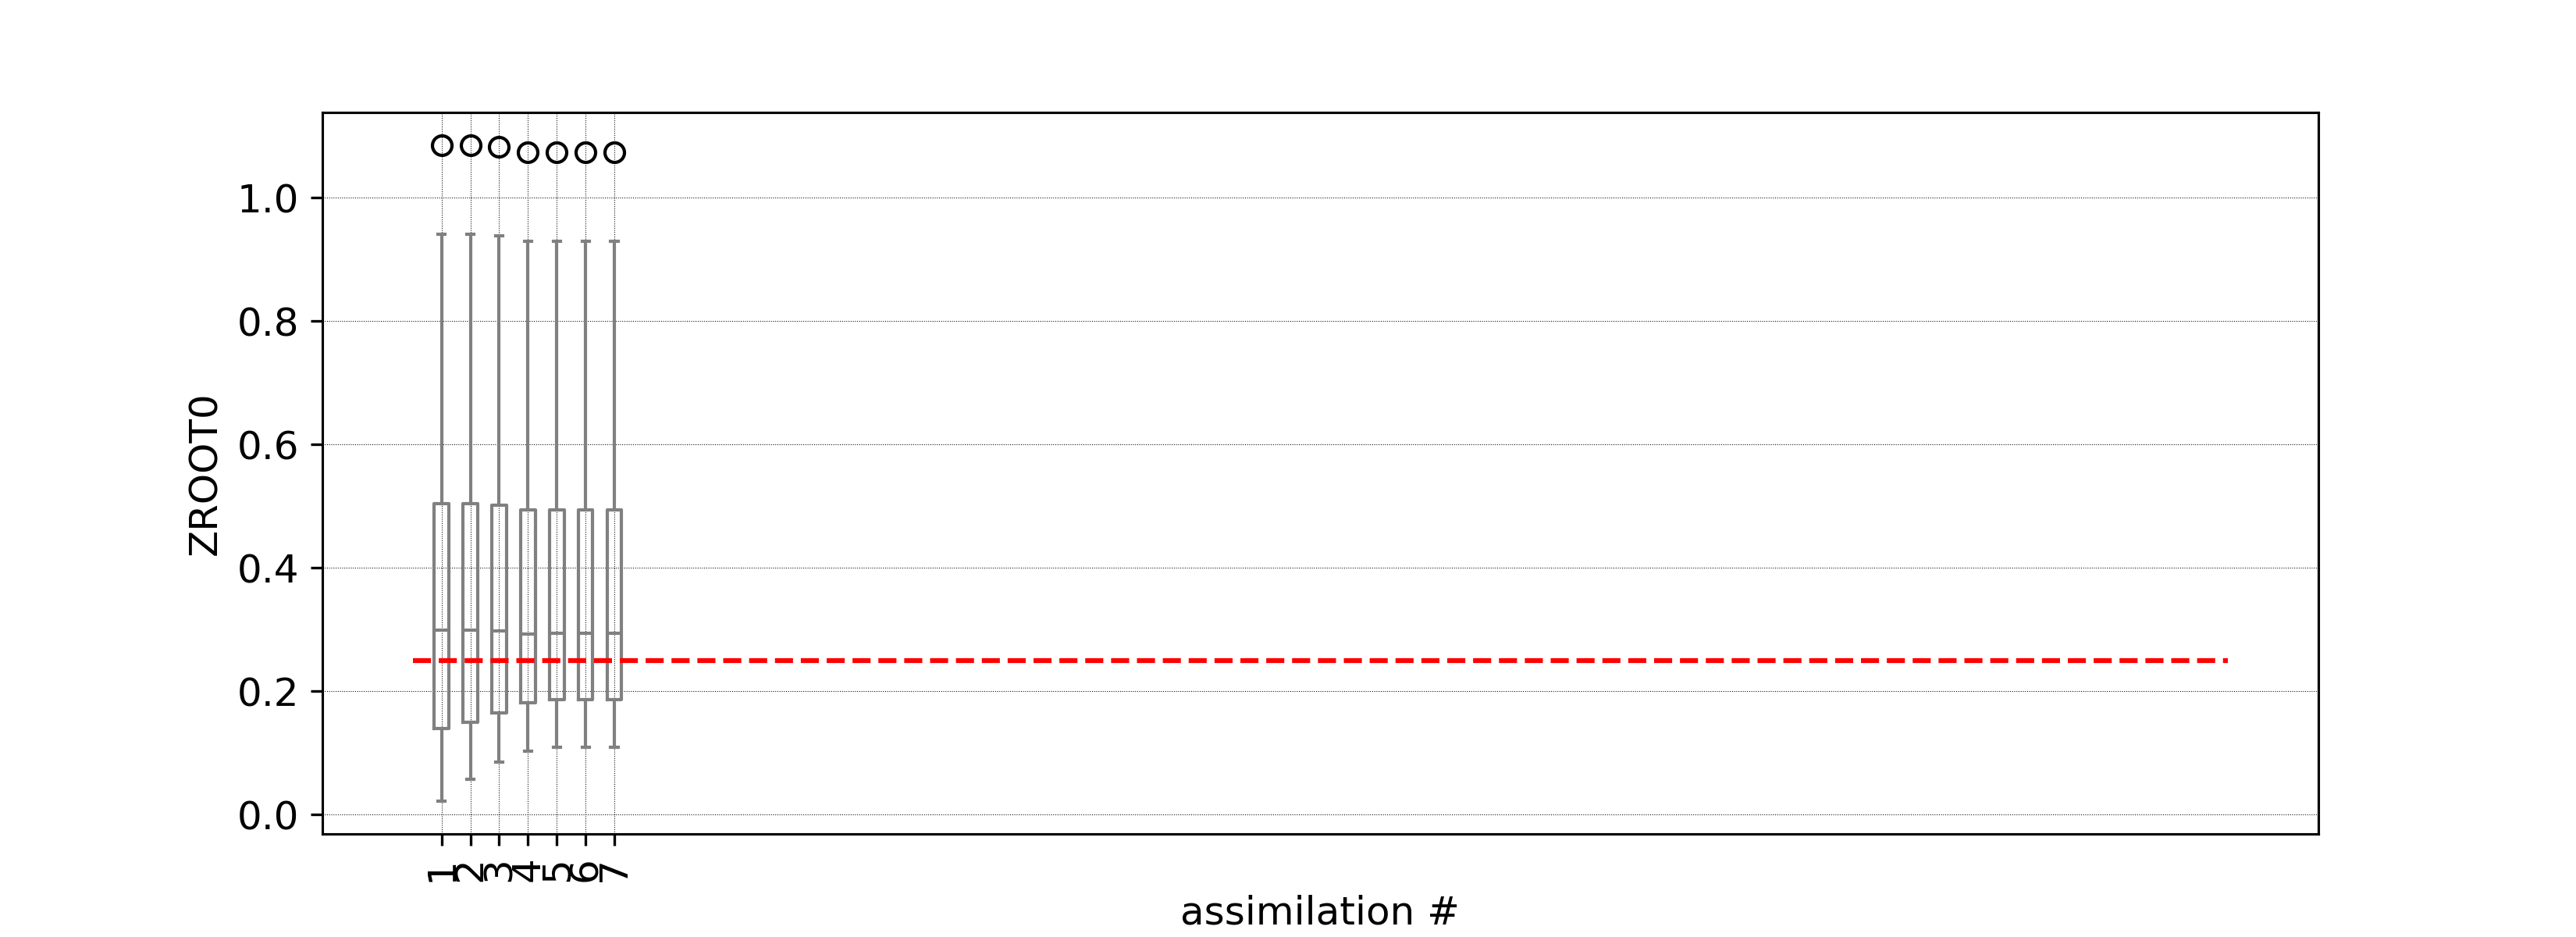
\includegraphics[width=0.75\linewidth]{files/ZROOT0-ce5733aa3f0f117411219fc58d49efb9.png}
\caption[]{ZROOT0}
\label{ZROOT0}
\end{figure}

\begin{figure}[!htbp]
\centering
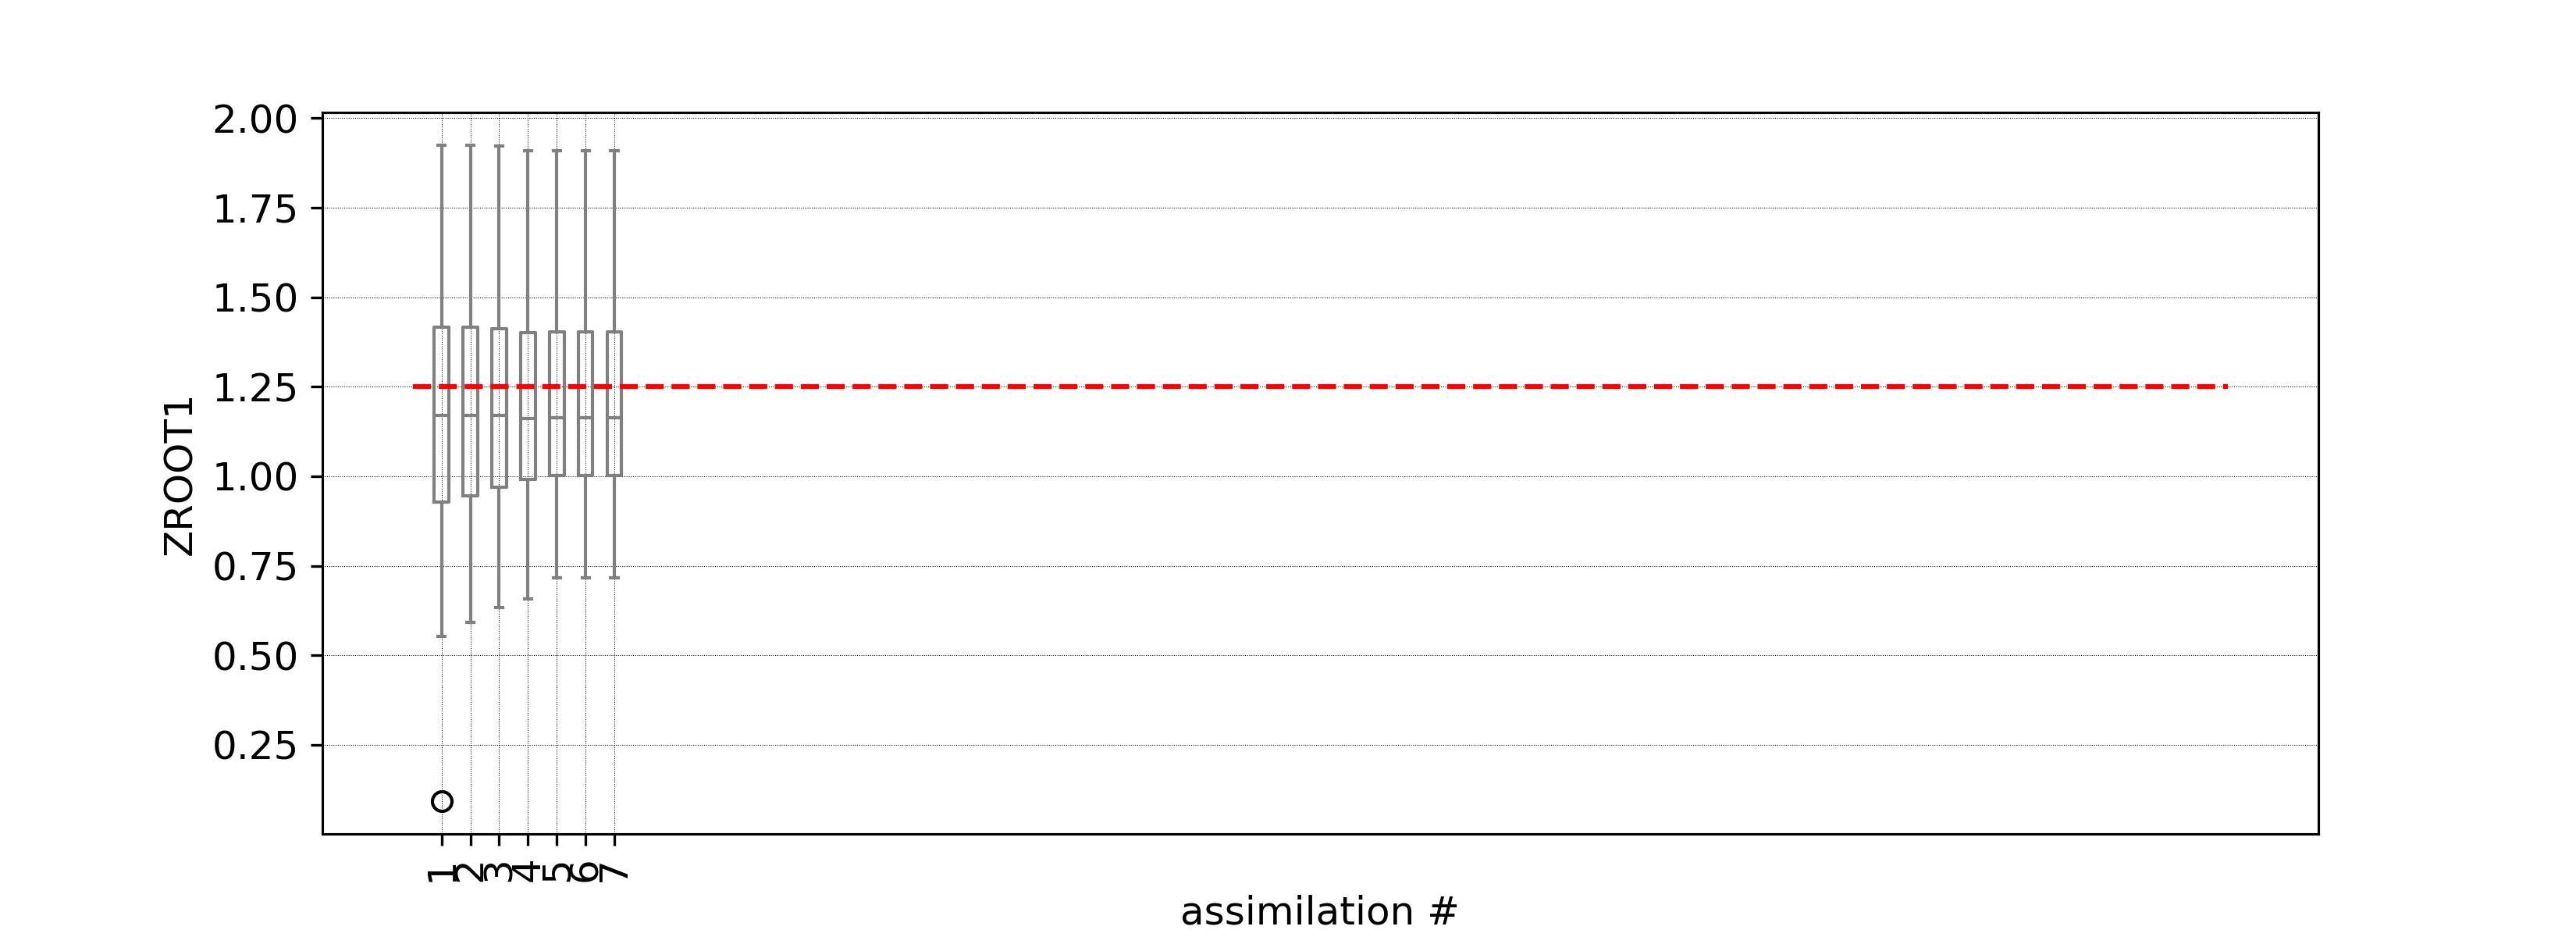
\includegraphics[width=0.75\linewidth]{files/ZROOT1-f9256fae2e44499ee733dbcf8297b225.png}
\caption[]{ZROOT0}
\label{ZROOT1}
\end{figure}
\end{document}
